\documentclass[11pt]{report} % DOKUMENTKLASSE. Mulighederne inkl. article, report, book, memoir  %
                              % Geometri-pakke: Styrer bl.a. maginer                              %
\usepackage[a4paper, hmargin={2.8cm, 2.8cm}, vmargin={2.8cm, 2.8cm}]{geometry}                    %
\usepackage{amssymb}          % Matematiske tegn og skrifttyper, bl.a. \mathbb{}                  %
\usepackage{amsthm}           % Opsætning der gør sætninger og beviser nemmere, se amsthdoc.pdf   %
\usepackage[utf8]{inputenc}   % Lidt kodning så der ikke kommer problemer ved visse konverteringer%
\usepackage[T1]{fontenc}      % Lidt kodning så der ikke kommer problemer ved visse konverteringer%
\usepackage{amsmath}          % Matematiske tegn                                                  %
\usepackage[colorlinks=true]{hyperref}   % Referencer som hyperlinks                              %
%\usepackage{txfonts}         % Times font                                                        %
\usepackage{graphicx}         % Graphicx pakke                                                    %
\usepackage{xparse}         % Graphicx pakke                                                    %
\usepackage{bigfoot}          % \verb in footnote                                                    %
\usepackage{caption}          % Caption-pakke                                                     %
\usepackage{subcaption}       % Subcaption-pakke                                                  %
\setlength{\captionmargin}{20pt}% Sætter caption-margin                                           %
\usepackage{listings}         % Listings. Indsætter kildekode pænt.                               %
\usepackage{float}            % Keeping figures in place                                          %
\lstset{                      %                                                                   %
  basicstyle=\ttfamily\footnotesize, % Sætter basisstilen i listings                              %
  showstringspaces=false,     % no special string spaces                                          %
  extendedchars=true,         % Bogstaver som æ, ø og å 
}                             %                                                                   %
\usepackage{verbatim}
\usepackage{enumitem}
\usepackage{courier}          % Courierskrifttype. Slankere skrivemaskineskrift i verbatim og     %
                              % listings                                                          %
\usepackage{multicol}         % Kolonner                                                          %
\usepackage[babel, titelside, nat, farve, en]{ku-forside}   % KU-forside med logoer               %
\def\HyperLinks{              % Hyperlinks-pakke, referencer til links og tillader links til www  %
\usepackage[pdftitle={\TITEL},pdfauthor={\FORFATTER}, % Et lille trick så pakken indlæses efter   %
pdfsubject={\UNDERTITEL}, linkbordercolor={0.8 0.8 0.8}]{}} %  titlen defineres.          %
\DeclareSymbolFont{rsfscript}{OMS}{rsfs}{m}{n} % Henter alfabet                                   %
\DeclareSymbolFontAlphabet{\mcal}{rsfscript} % Kalder dette alfabet for \mcal                     %
\setlength\arraycolsep{2 pt}  % Sætter kolonneafstanden i tabeller og eqnarrays til 2pt           %
\setcounter{tocdepth}{3}      % Dybde af indholdsfortegnelsen,                                    %
                              % 1 resulterer i kun sections kommer med, 2 er secs og subsec. etc  %
% \setcounter{secnumdepth}{0}   % Dybde af sektionsnummereringen.                                   %
%%%%%%%%%%%%%%%%%%%%%%%%%%%%%%%%%%%%%%%%%%%%%%%%%%%%%%%%%%%%%%%%%%%%%%%%%%%%%%%%%%%%%%%%%%%%%%%%%%%
\titel{Evaluating throughput scalability of multi-core} %                 %
\titelto{in-memory hash indices} %                 %
\undertitel{Faculty of Computer Science} %                                                        %
\opgave{Thesis Report}                   % Findes kun under 'titelside' muligheden i ku-forside   %
\forfatter{Jakob Hanehoj}                %                                404                        %
\dato{\today}                            %                                                        %
\vejleder{Marcos Antonio Vaz Salles and Vivek Shah} % Findes kun under 'titelside' muligheden i KU-forside   %
\HyperLinks                              % Sætter pdf-titel til at svare til de just definerede   %
                                         %                                                        %
\newsavebox{\fminipagebox}
\NewDocumentEnvironment{fminipage}{m O{\fboxsep}}
 {\noindent\begin{lrbox}{\fminipagebox}
  \begin{minipage}{#1}\ignorespaces}
 {\end{minipage}\end{lrbox}%
  \noindent\fcolorbox{black}{used_grey}{\makebox[#1]{%
    \kern\dimexpr-\fboxsep-\fboxrule\relax%
    \usebox{\fminipagebox}%
    \kern\dimexpr-\fboxsep-\fboxrule\relax%
  }}%
 }
\definecolor{used_grey}{rgb}{0.8, 0.8, 0.8}
\definecolor{used_blue}{rgb}{0.8, 0.8, 0.2}
\definecolor{used_red}{rgb}{0.2, 0.8, 0.4}
\newsavebox{\globalminipagebox}
\NewDocumentEnvironment{globalminipage}{m O{\fboxsep}}
 {\par\kern#2\noindent\begin{lrbox}{\globalminipagebox}
  \begin{minipage}{#1}\ignorespaces}
 {\end{minipage}\end{lrbox}%
  \noindent\fcolorbox{used_red}{used_red}{\makebox[#1]{%
    \usebox{\globalminipagebox}%
  }}\par\kern#2
 }
\newsavebox{\localminipagebox}
\NewDocumentEnvironment{localminipage}{m O{\fboxsep}}
 {\par\kern#2\noindent\begin{lrbox}{\localminipagebox}
  \begin{minipage}{#1}\ignorespaces}
 {\end{minipage}\end{lrbox}%
  \noindent\fcolorbox{used_blue}{used_blue}{\makebox[#1]{%
    
    \usebox{\localminipagebox}%
    
  }}\par\kern#2
 }

\begin{document}                         %                                                        %
\maketitle % Laver titlen                %                                                        %
                                         %                                                        %
%%%%%%%%%%%%%%%%%%%%%%%%%%%%%%%%%%%% Indholdsfortegnelse %%%%%%%%%%%%%%%%%%%%%%%%%%%%%%%%%%%%%%%%%%

\begin{abstract}
asdasdsad
\end{abstract}
\tableofcontents % indholdsfortegnelsen                                                           %
\listoffigures  % Liste over figurer \begin{figure} ... \end{figure}                              %
%%%%%%%%%%%%%%%%%%%%%%%%%%%%%%%%%%%%%%%%%%%%%%%%%%%%%%%%%%%%%%%%%%%%%%%%%%%%%%%%%%%%%%%%%%%%%%%%%%%

\chapter{Introduction}
\label{chap:introduction}

\chapter{Background}
\label{chap:background}
In recent years there has been a lot of research in the field of key-value stores, primarily focused on improving the performance of these systems. Since key-value stores manage underlying index structures, an area of research in this field has been to optimize the performance of index structures. \\
\\
Due to in increase in main memory size and affordability, much of the recent research has been on in-memory index structures, which store the entire data structure in main memory, thus removing the high cost of accessing disk. Likewise, the increasing amount of cores in modern hardware has lead to an increased effort in research on multi-core index structures. \\
\\
Most of the recent research on in-memory multi-core index structures has been analyzing ordered data-structures, such as trees. However, there is strong evidence that hash indices are much faster than the most recent and best tree-structured indices. The goal of this project is thus evaluating the performance of multi-core in-memory hash indices, with respect to a key-value store setting. \\
\\
We first present a brief background on key-value stores in Section~\ref{sec:background_key_value_store}, in order describe the setting in which the index structures are intended to be used. Next, we present relevant background information on hash functions in Section~\ref{sec:background_hashing_algorithms}, yielding an overview of important characteristics of the hash functions used in this project. Then we present relevant background information on hash indices in Section~\ref{sec:background_hashing_indices}, which provides a basis for the project to build upon. Finally, we give a brief introduction to the framework used for evaluating the built hash indices in Section~\ref{sec:background_ycsb}.
\section{Key-value stores and index structures}
\label{sec:background_key_value_store}
A key-value store is a simple database management system based on associative arrays, used to store, retrieve and manage index structures. These index structures are fundamental data structures that contain a collection of key-value pairs, thus associating a unique key with a single value. The index structures yield a direct mapping from any possible key to a given position in the data structure, which in turn yields fast access to the data. The performance of the index structure does therefore heavily affect the performance of the key-value store, in which it is used.\\
\\
Both key-value stores and their index structures adhere to the basic \verb|CRUD| API, which defines the following four operations:
\begin{itemize}
  \item \verb|C|reate, for inserting a key-value pair in the store
  \item \verb|R|ead, for retrieving a key-value pair from the store
  \item \verb|U|pdate, for editing existing values in the store
  \item \verb|D|elete, for removing a key-value pair from the store
\end{itemize}
\noindent
Additionally, some key-value stores support range-scans internally, used for retrieving a range of key-value pairs, where some implementations of range scans are ordered, thus yielding sorted results, while others are unordered, yielding results in the order they were found.\\
\\
There are many well known examples of key-value stores, where some of the most popular examples are Redis~\cite{redis}, Cassandra~\cite{cassandra}, Oracle NoSQL Database~\cite{oracle}, HBase~\cite{hbase}, Dynamo~\cite{dynamo} and memcached~\cite{memcached}. Out of all of these only memcached is an in-memory key-value store, which does not focus on multi-core performance. However, recently a new multi-core in-memory key value store has been presented, namely Masstree~\cite{MT12}. \\
\\
Masstree is an ordered multi-core key-value store, which is specialized for usage when all data fits in main-memory. Its index structure is a trie-like concatenation of B$^+$-trees, and it provides a flexible data storage model, by handling variable length keys, including keys with long common prefixes~\cite{MT12}. \\
\\
By combining these fundamental concepts in a key-value store, Masstree has shown superior performance compared to many of the most popular key-value stores, including redis, the most popular key-value store currently~\cite{db_ranking}. This which emphasizes the strength of multi-core in-memory key value stores. By combining the superior results of Masstree with the fact that there is strong evidence that hash indices are faster than even the best tree-structured indices~\cite{RAD15}, we have found it interesting to evaluate how well multi-core in-memory hash indices perform.\\
\\
The topic of this project is thus an evaluation of the performance of multi-core in-memory hash indices. As for most key-value store performance evaluations, the performance metric measured is throughput, i.e., queries per second. However, since we are specifically targeting a multi-core setting, there is also much focus on evaluating the scalability of throughput across multiple cores. Additionally, in order to provide a flexible data storage model, we concentrate on hash indices that can handle variable length bit string keys efficiently, and include support for ordered range scans.\\
\\
Since we are evaluating hash indices, thus not key-value stores, the goal of the project is a better understanding of the performance impact of important choices to be made, when choosing and tuning an multi-core in-memory hash index for a key-value store, rather than a comparison to known key-value store implementations. The evaluation is based on the YCSB benchmark~\cite{BC10}, as this is a commonly used standard for evaluating the performance of data stores.

\section{Hash functions}
\label{sec:background_hashing_algorithms}
The space of hash functions is vast, spanning over many different ideas for mapping arbitrary data into fixed sized data. In this section, hash functions relevant for the project are presented. We start by presenting an overview of the relevant hash functions in Section~\ref{subsec:background_review_of_hashing_algorithms}, to provide an understanding of our motives for our choices of hash functions. This is followed by a fundamental presentation of each of the hash functions in Sections~\ref{subsec:background_simple_tabulation_hashing} and~\ref{subsec:background_murmur_hashing}, to give an understanding of their key concepts.
\subsection{Overview of hash functions.}
\label{subsec:background_review_of_hashing_algorithms}
In our selection process of hash functions for this project, certain theoretical properties have been important. Firstly, the hash function should be able to handle variable length keys efficiently, as such keys are in focus in this project. Hash functions designed for fixed length keys could be adapted to handle arbitrary length keys, by padding the keys with 0's. However, such an implementation would not yield efficient memory usage, as all keys would have to be padded to the length of the longest key. Therefore, we have chosen to focus on algorithms which are designed to be able to handle variable length keys. \\
Secondly, the hash function should be robust to skewed input distribution, yielding a close to uniform output distribution regardless of the input distribution. Lastly, since the project focuses on throughput of the hash indices, the computational complexity of the underlying hash functions should be lowest possible.\\
\\
One such hash function is found in simple tabulation hashing, which handles variable length keys and is simple both in terms of computational complexity and implementation, while being very robust. The tabulation hash function is by no means a new form of hashing, as the first instances of tabulation hashing was published in 1970 by Albert Zobrist~\cite{Zobrist}, and the method was later extended in greater generality by Carter \& Wegman in 1979~\cite{WC79}. \\
\\
A common measurement for robustness of a hash function is $k$-independence, originally defined by Wegman and Carter under the name "strongly universal$_k$ hash family"~\cite{WC81}. A more recent equivalent definition of $k$-independence of family of a hash function $H = {h : U \rightarrow [m]}$ is given by the following two conditions:
\begin{itemize}[nolistsep]
  \item for any fixed $x \in U$, as $h$ is drawn randomly from $H$, $h(x)$ is uniformly distributed in $[m]$.
  \item for any fixed, distinct keys $x_1,...,x_k \in U$, as $h$ is drawn randomly for $H$, $h(x_1),...,h(x_k)$ are independent random variables.
\end{itemize}
Higher degrees of $k$-independence yield certain guarantees for the given hashing function. Simple tabulation hashing is 3-independent, while better implementations of tabulation-based methods can supply 5-independence~\cite{TZ09}. Pătraşcu and Thorup have recently shown that despite the low independence of simple tabulation hashing, it can be shown to provide many of the guarantees provided by higher independence~\cite{PT11}, yielding strong statistical properties for a very simple hashing method. Additionally, they have proven that tabulation hashing with linear probing can achieve $O(1)$ complexity for insertions, deletions, and lookups. Overall, this makes tabulation hashing interesting for this project.\\
\\
The interest in tabulation hashing even more emphasized by a recent thorough comparison of hash functions, performed by Richter et al.~\cite{RAD15}, in which they evaluate four hash functions, namely
\begin{itemize}
\item Multiply-shift hashing
\item Multiply-add-shift hashing
\item Murmur hashing
\item Tabulation hashing
\end{itemize}
\noindent
Since multiply-shift hashing and multiply-add-shift hashing only have implementations for fixed-length keys, we have chosen to focus on murmur hashing and tabulation hashing. Richter et al. conclude that both of these hashing methods are slower than both multiply-shift hashing and multiply-add-shift hashing, even though both have greater robustness in terms of distributional properties, when faced with skewed input distributions. Between murmur hashing and tabulation hashing, they conclude murmur hashing to be the faster, with tabulation hashing being the most robust. \\
\\
Tabulation hashing and murmur hashing has therefore been chosen as the hash functions evaluated in this project. In the following two sections, these two hash functions are presented.
\subsection{Simple tabulation hashing}
\label{subsec:background_simple_tabulation_hashing}
Tabulation hashing is a hashing scheme that combines table lookups and \verb|xor| operations in order to calculate the hash value, an bit string of a chosen size. It views a key \emph{x} as a vector of \emph{c} same size characters $x_1, ..., x_c$, and relies on one table $T_i$ for each of the \emph{c} character positions. The tables contain truly random bit strings,\footnote{E.g. drawn from random.org, as suggested by Pătraşcu and Thorup} of the size of the wanted hash value. The hash function simply performs a lookup for each character in the corresponding table, and \verb|xor| the lookup results together:
$$h(x) = T_1[x_1] \oplus ... \oplus T_c[x_c]$$
The lookups are done by interpreting each character as an integer and using this integer to index into the corresponding table. The tables does therefore contain $2^{|x_i|}$ entries, which are initialized prior to execution of the hash function. This makes the complexity of the algorithm only depend on the speed of the table-lookups and the \verb|xor|'ing. By constructing the table small enough to fit in fast cache, the table lookups become very efficient, making the algorithm very fast while also being straightforward to implement.\\
\\
The size of the characters influences both the space used and the runtime of the algorithm. If drawing keys from a universe of size \emph{u}, we see that we have $O(u^{1/c})$ entries in each table, making the total amount of entries become $O(cu^{1/c})$.\footnote{Example: Drawing a key of from the 128 bit universe \emph{u} and using a character size 8 bits yields $128/8=16$ characters, thus also 16 tables. Each of the tables will have to contain entries for the $2^8$ different combinations of a given character, thus containing $2^8 = 2^{128/16} = (2^{128})^{1/16} = O(u^{1/c})$ entries in each table. For \emph{c} characters we use \emph{c} tables, thus a total amount of entries becomes $O(cu^{1/c})$.} Since the \emph{c} in the exponent outweighs the factor \emph{c}, the total space required for the tables is decreased as the amount of characters is increased. Thus, in order to ensure that the tables can fit in fast cache (optimally \verb|L1|-cache), the size of the character could be decreased. \\
\\
However, decreasing the size of the character yields more characters, which in turn yields more lookups and more \verb|xor| operations, thus increasing the runtime of the algorithm. The decision of a good character size is therefore a trade-off between having small enough characters for the tables to fit in fast cache, while not having too small characters to avoid too many computations.\\
\\
An example of a hashing could be as following:\\ Assuming we get a key of size six bits (i.e. \verb|101100|) and use a character size of two bit, we get three characters, thus also three tables, each with four entries. In this example, the hash value type has been defined as an bit string of length eight, meaning that all the values in the tables also are bit strings of length eight. Three tables have been defined as seen in Figure \ref{fig:tabulation_tables}.\\
\begin{figure}
  \quad\quad\quad\quad\quad
  \begin{tabular}{|c|c|}
  \hline
  \multicolumn{2}{|c|}{Table 1}\\
  \hline
  00&01010110\\
  01&11010011\\
  10&00111011\\
  11&10101101\\
  \hline
  \end{tabular}
  \quad\quad\quad\quad
  \begin{tabular}{|c|c|}
  \hline
  \multicolumn{2}{|c|}{Table 2}\\
  \hline
  00&11001100\\
  01&00111001\\
  10&11011001\\
  11&11000101\\
  \hline
  \end{tabular}
  \quad\quad\quad\quad
  \begin{tabular}{|c|c|}
  \hline
  \multicolumn{2}{|c|}{Table 3}\\
  \hline
  00&10100111\\
  01&00101100\\
  10&01011001\\
  11&01010101\\
  \hline
  \end{tabular}
  \caption{Example of tabulation tables}
  \label{fig:tabulation_tables} 
\end{figure}
\noindent\\
The hash function is then found by splitting the key into the three characters, each of size two bits: $$x_1 = 10, x_2 = 11, x_3 = 00$$ Using these characters as index into their corresponding tables yield the following lookup values: $$T_1[x_1] = 00111011,\ \ \ \ T_2[x_2] = 11000101,\ \ \ \ T_3[x_3] = 10100111$$ Finally, \verb|xor|'ing these lookup values together yield the hash value: $$00111011 \oplus 11000101 \oplus 10100111 = 01011001$$
The final hash value of this example is therefore \verb|01011001|.
\subsection{Murmur hashing}
\label{subsec:background_murmur_hashing}
Murmur hashing is one of the most commonly used general purpose hash function, which is composed of several multiplications (MU) and rotations (R), thus creating the name (MU)(R)(MU)(R)~\cite{Mur3}. It takes a key of any size, and splits it up into sections of the wanted hash value size. Currently, implementations for 32bit and 128bit hash values exist, causing sections of either 32bit or 128bit to be used. For each of these sections multiplications with statically defined values and rotations are performed. The rotations are essentially circular shifts, where the \verb|r| most significant bits are made the least significant bits, while the remaining bits are shifted to be the most significant bits.\\
\\
\begin{fminipage}{\linewidth}
\begin{lstlisting}
  int rotl32 (int x, int r ) {
    return (x << r) | (x >> (32 - r));
  }
\end{lstlisting}
\end{fminipage}
\vphantom{fill}\\
Finally, any remainder of the key which doesn't fit into exact section (i.e. the tail of the key) is included by a the murmur finisher~\cite{Mur3}, which uses shifts and multiplications with statically defined values.\\
\\
Thus, the algorithm only uses $O(1)$ operations, yielding a low computational complexity, while also yielding good distributional properties~\cite{RAD15}.
\section{Hash indices}
\label{sec:background_hashing_indices}
Hash indices are fundamental index structures in computer science. Like key-value stores, hash indices also expose the basic four operations of \verb|get|, \verb|insert|, \verb|update| and \verb|remove|. Additionally, some implementations also expose \verb|range scans|. \\
\\
In the following sections, we will first present the relevant literature on hash indices, then present the details on the chosen hash indices individually, and finally briefly summarize the key concepts of radix partitioning, which is needed for partitioning of hash indices, described in Section \ref{sec:design_partition_hash_index}

\subsection{Overview of hash indices}
\label{subsec:background_review_of_hash_indices}
Hash indices distribute data entries among a set of slots, while relying on a scheme for solving collisions in the slots. One of the simplest and most effective collision resolution schemes is chained hashing, in which collisions are resolved by placing all data entries of the same slot in some container, or chain. A common implementation of this strategy uses linked lists, as they are simple to implement and maintain. In this case, all operations can be solved by following or modifying pointers. \\
\\
In the survey made by Richter et al.~\cite{RAD15}, they also include an analysis of five different hash indices, namely
\begin{itemize}
  \item Chained hashing
  \item Linear probing
  \item Quadratic probing
  \item Robin Hood Hashing on LP
  \item Cuckoo Hashing
\end{itemize}
They have shown that chained hashing is very resilient to unsuccessful queries,\footnote{I.e., queries where the searched key is not present in the data structure.} while providing overall good average case performance. One of the reasons that the performance of chained hashing is worse than other hash indices under certain circumstances is the poor cache utilization using linked lists yields. This is due to new memory areas that will have to be loaded into the cache repeatedly. Additionally, the random memory jumps makes data-prefetching difficult for the hardware. For in-memory uses, these two disadvantages become quite significant. \\
\\
Askitis and Zobel have addressed this issue by replacing the linked lists with dynamic arrays, in what they called array hashing \cite{NA09, AJ05}. They have shown that the obvious disadvantage of resizing the arrays dynamically is heavily outweighed by the advantages of better cache utilization and data prefetching in an in-memory setting. Additionally, using an array instead of linked lists yields better space utilization, as the overhead from nodes and pointers is eliminated. \\
\\
In their most recent study, Askitis and Zobel specifically addressed implementing this version of chained hashing for integer-type hash values, and compared it to linear probing, bucketized cuckoo hashing and clustered chained hashing.\footnote{Bucketized cuckoo hashing and clustered chained hashing are both adaptations of their regular implementations, which try to improve cache utilization by placing a given amount of entries in a local memory region (bucket or cluster), thus offering some of the same advantages of array hashing over their regular counterparts} \\
\\
Array hashing was found to be generally faster than bucketized cuckoo hashing and clustered chained hashing for all operations~\cite{NA09}. Linear probing was found to be the fastest in all but one situation; when the allocated data structure is sufficiently large. The requisite data structure size is however often difficult to estimate, which either leads to excessive space usage, making linear probing very inflexible, or exhibits bad performance. Contrarily, array hashing is able to efficiently handle greater loads. \\
\\
Finally, Dudás and Juhász have shown great multi-core scalability results for array hashing, using a lock-free structure~\cite{ADSJ13}. We have therefore found array hashing promising, and chosen to work on this structure. \\
\\
A dual to the chained hashing is found in extendible hashing~\cite{dms03}, which yields an upper limit on the probing time for all of the four operations (excluding range scans), making extendible hashing interesting for evaluation. Therefore, we will also be working with extendible hashing.
\subsection{Chained hashing using arrays}
\label{subsec:background_chained_hashing_using_arrays}
The chained hashing data structure is based on the concept of a directory containing buckets~\cite{ItA092}. The buckets are dynamically sized containers of data entries, and each data entry only contains its key and value.
The size of the directory is always fixed, meaning that there will not be any instantiation of additional buckets. Instead, chained hashing extends the individual buckets as they fill up. \\
\\
In array hashing, the bucket containers are implemented using arrays. Due to the statically allocated size of arrays, this implementation needs to handle the underlying memory management of insert and delete operations more carefully than the linked list implementation, i.e., by handling reallocation of the arrays. This careful memory management causes a performance drawback. The gain on the other hand comes from the efficient accessing capabilities of the arrays, as well as better cache utilization and data prefetching.\\
\\
The predefined size of the directory is always chosen to be a power of 2, referred to as the directory depth (\verb|dir_depth|), since this means that all the buckets can be enumerated using a given amount of bits.\footnote{Example: Choosing the directory depth to be 16 yields a directory of size $2^{16} = 16384$, thus containing 16384 buckets. As such, each combination of \verb|dir_depth| bits enumerates a unique bucket.} Thus, all of the operations (except the range scans) have in common that they locate the correct bucket for the key, by hashing the key to its hash value and looking at \verb|dir_depth| least significant bits of this hash value. \\
\\
Common for the four operations \verb|get|, \verb|update|, \verb|insert| and \verb|remove| is that they all find the bucket in which the operation is to be performed by hashing the key using the hash function, and then use the \verb|dir_depth| least significant bits of the hash value as an index into the directory. Once the correct bucket has been found, the individual operations proceed as described in the following paragraphs.

\paragraph{Get.} Once the correct bucket has been located, the lookup is performed by iteratively comparing the key of each data entry inside the bucket with the given key. If a match is found, the value of the data entry is returned and the lookup succeeds; otherwise, the next key is compared. If the end of a bucket is reached without finding a matching key, the lookup fails. 

\paragraph{Update.} Updates are performed similarly to lookups, except that instead of returning the value of the correct data entry (if found), the value is updated to the new value. 

\paragraph{Insert.} Insertion is performed by locating the correct bucket, and placing the data entry at the first available slot. As for all separate chaining hashing variants, insertion into a full bucket is done by increasing the size of the bucket, thus here we increase the size of the array, which in turn might require a reallocation of the array. It is common practice to double the size of the array whenever an increase in size is required, as this eliminates situations where the array grows repeatedly, causing many expensive reallocation operations to be done in succession~\cite{DPH90}. \\
\\
However, Askitis suggests that singular increases of the arrays are used, as they have found no significant performance increase when compared with size-doubling~\cite{NA09}. This effect is emphasized by Dudás and Juhász, who also increase the size by one every time, but do so by allocating a new array of size one larger, in order to be able to use CAS operations for synchronization~\cite{ADSJ13}. \\
\\
Using the approach of singular increase, the arrays will always be completely full, and thus not waste  memory. This does, however, also mean that any insert into the hash index will cause an increase of the size of a bucket, potentially causing many successive reallocation operations. 

\paragraph{Remove.} Removal is also done by finding the correct bucket in the directory, iteratively comparing the key of each data entries in the bucket with the given key, and removing the data entry if it is present. As for insertion, it is also suggested by Askitis that a removal decrements the size of the array, in order to avoid having empty slots in the array~\cite{NA09}. He did this by shifting all entries succeeding the found entry one slot towards the beginning, leaving the last slot empty to be removed. 

\paragraph{Range scans.} Range scans are handled quite differently from the other four operations, as they operate multiple buckets. Since array hashing is an unordered data structure, scans for ranges of keys are not easily supported. In order to find all keys in a given range, a complete search of the entire structure must be performed by running through all entries in the hash index, and comparing them to the given range. This procedure certainly finds all the correct entries, but might be very slow, especially when searching for small range. The computational complexity of finding all the entries in the range is always $O(entry\_amount * probe\_time)$, irrespective of the size of the range. \\
\\
In this case of small ranges, it might be more useful to simply rehash every key in the searched range to obtain its bucket location, and search for it in the given bucket. In this way, the computational complexity of finding all the entries in the range becomes dependent on the size of the range, i.e., \verb|O(range_length * (hash_time + probe_time))|. The probing time is always constant, which makes this solution good for small ranges, but for longer ranges, the increased time caused by the additional hashing might take over, causing this to be worse than the full search. This procedure does also require for the key-type to be enumerable, as one would have to iterate over all keys between the start- and end-key. As we are using strings, this is not the case, making this solution unfeasible.

\subsection{Extendible hashing}
\label{subsec:background_extendible_hashing}
A dual approach to array hashing is found in extendible hashing~\cite{dms03}, which uses the same key components as array hashing, namely a directory of buckets, which in turn hold the data entries. However, in extendible hashing, the directory can be seen as a dynamically sized array, which from start-up is quite small, but which will grow when needed.\footnote{Some implementations also allow the directory to shrink under certain circumstances.} The buckets of extendible hashing are fixed-sized containers for the data entries, and all buckets have the same predefined size. Additionally, in extendible hashing, the directory contains pointers to buckets, instead of the buckets themselves, which yields an optimized algorithm for the growth of the directory, as we shall see later in this section.\\
\\
To describe the current size of the directory, a \verb|global_depth| denotes how many bits are needed to enumerate every bucket pointer in the directory. The maximum amount of buckets in the directory is therefore always $2^{(global\_depth-1)}$. Thus, to find the correct bucket for a given hash value, one follows the pointer whose position in the directory is equal to the \verb|global_depth| least significant bits of the hash value.\\
\\
When the directory has to grow (more on when this happens later), we simply double its size, increment the \verb|global_depth|, and create a copy of every bucket pointer, stored in the newly allocated second half of the directory. The increase in \verb|global_depth| includes another least significant bit of the hash value, which is then used to distinguish between the original pointers and the newly copied pointers, where a 0 yields the old pointer, and a 1 yields the copy. Note that this directory increase does not create any new buckets, but simply allows for twice as many buckets to be stored when needed. We therefore end up with (at least) two pointers to each bucket, directly after the doubling of the directory. An example of this directory doubling can be seen in Figure~\ref{fig:global_depth_increase}.\\

\begin{figure}[H]
  \centering
  \includegraphics[width=0.8\textwidth]{Graphs/global_depth_increase.png}
  \caption{Doubling of the directory for extendible hashing}
  \label{fig:global_depth_increase}
\end{figure}
\noindent
In Figure~\ref{fig:global_depth_increase}, we see the directory in blue, originally with a \verb|global_depth| of two, thus containing four entries. Additionally, we have four buckets in red (A, B, C, D).\footnote{The buckets has been color coded, and all pointers pointing to the given bucket has been given the same color, for ease of understanding.} After the growth of the directory, the \verb|global_depth| is increased to three, which causes twice as many bucket pointers to be present. Each new pointer is a copy of an old one, thus pointing to the same bucket (indicated with dashed arrows of the same color). Notice that there has been no new allocations of buckets.\\
\\
Thus, a bucket can be pointed to by multiple entries in the directory, as long as they have a common set of least significant bits. An individual \verb|local_depth|\footnote{The yellow boxes in Figure \ref{fig:global_depth_increase}} is stored in each bucket, which denotes how few bits of a hash value are sufficient to uniquely identify the given bucket. The \verb|global_depth| must always be kept at least as high as the \verb|local_depth| of any bucket, as the bucket would otherwise require more bits to be uniquely identified than what is used to identify buckets in the directory. \\
\\
In Figure \ref{fig:global_depth_increase} it can be seen that all buckets have a \verb|local_depth| of two. After doubling the directory, all pointers going in to a given bucket shares the \verb|local_depth| least significant bits in the directory. \\
\\
The difference between the \verb|global_depth| and a bucket \verb|b|'s \verb|local_depth| denotes how many pointers in the directory are pointing to \verb|b|, since this difference corresponds to the bits that, in addition to the least significant bits required to uniquely identify \verb|b|, are used to identify the pointer in the directory. Each combination of these \verb|global_depth - b.local_depth| bits yield a new pointer, which points to \verb|b|, and thus we have $2^{(global\_depth-b.local\_depth)}$ pointers pointing to \verb|b|. \\
\\
These additional bits has been illustrated in Figure \ref{fig:global_vs_local}, indicated by a red box. 
\begin{figure}[H]
  \centering
  \includegraphics[width=0.7\textwidth]{Graphs/Global_vs_Local.png}
  \caption{Illustration of difference in global and local depth}
  \label{fig:global_vs_local}
\end{figure}
\noindent
Since the difference in \verb|global_depth| and the \verb|local_depth| of each bucket is two, all buckets have $2^2 = 4$ pointers pointing to them. The four pointers of each bucket all have two common least significant bits, while the additional bits are unique for each pointer.\\
\\
In extendible hashing, the pointer to the correct bucket for the four operations \verb|get|, \verb|insert|, \verb|update| and \verb|remove| is found by hashing the key using the hash function, and using the \verb|global_depth| least significant bits of the hash value as an index in the directory. Once the correct bucket has been found, the individual operations proceed as described in the following paragraphs. \\
\\
Additionally, since the extendible hashing primarily deviates from array hashing in the way it handles full buckets, only the two operations that change the amount of entries in the data structure (namely \verb|insert| and \verb|remove|) are significantly different from array hashing implementation. Thus, the \verb|get|, \verb|update| and \verb|range-scan| operations are performed exactly as in array hashing, and are therefore not presented here.
\paragraph{Insert.} For inserts, an empty entry in the correct bucket is searched for. If such empty entry is present, the data entry is simply inserted there, and the insertion is finished. \\
\\
However, when a data entry insertion is attempted into a full bucket, a collision occurs, which requires additional space to be found. This space is found by splitting the bucket into two, amongst which the entries in the original bucket and the new entry to be inserted are redistributed. To distinguish between the original bucket and the new 'image bucket', an additional least significant bit is used, such that hash values for which the additional bit is 0 remain in the old bucket, while hash values for which the additional bit is 1 are moved to the new bucket. \\
\\
This inclusion of an additional bit is simply done by increasing the \verb|local_depth| of both buckets. By increasing the \verb|local_depth| of the original bucket, we also denote that fewer pointers should be pointing to the bucket, as only the pointers for whom their position in the directory has a (\verb|local_depth|+1)th least significant bit of 0, should be pointing to the original bucket, while the other half of the pointers should be pointing to the new image bucket.\\
\\
An example of this splitting of buckets can be seen in Figure \ref{fig:bucket_split}.
\begin{figure}[H]
  \centering
  \includegraphics[width=0.8\textwidth]{Graphs/Bucket_split.png}
  \caption{Splitting of a full bucket}
  \label{fig:bucket_split}
\end{figure}
\noindent
In Figure~\ref{fig:bucket_split}, we start by having four buckets, and all buckets have a capacity of four entries. Some entries have been inserted into the system, which are indicated by their hash values (i.e. the small numbers inside the boxes). \\
\\
Assume that an insertion of a key with hash value 20 is attempted. Since the \verb|global_depth| is equal to three, to find the correct bucket pointer, we evaluate the three least significant bits of 20, which yields four. We then follow the pointer at index four in the directory, which points to bucket \verb|A|. \\
\\
Since bucket \verb|A| is full, we have to split the bucket, thus creating a new bucket \verb|A2|. For both the original bucket \verb|A| and the newly created 'image bucket' \verb|A2|, the \verb|local_depth| is increased to three. With the increased \verb|local_depth| the pointers previously pointing to bucket \verb|A| must be redistributed between \verb|A| and \verb|A2|, based on the newly included third bit. \\
\\
Next, we also reallocate all the entries in bucket \verb|A| between the two new buckets, by looking at the newly included third bit. For the two entries with hash values 4 and 12, the third bit is 1, and therefore these entries are placed in the the image bucket. For the entries with hash values 32 and 16, the third bit is 0, so these two entries stay in the original bucket. \\
\\
Finally, we retry the insertion of the entry with hash value 20, and see that there is an available spot in bucket \verb|A2|, which the pointer at index four now is pointing to. This concludes the split of the bucket.\\
\\
Thus, insertion into a full bucket \verb|b| with \verb|local_depth| \verb|ld| is done by the following procedure.\\
\\
\begin{fminipage}{\linewidth}
\begin{lstlisting}[escapechar=@]  % Start your code-block

  1 Create new empty bucket i, with same local_depth as b, thus equal to ld;
  2 Insert i in directory, @$2^{ld}$@ positions after b.
  3 Increment b.local_depth and i.local_depth to ld+1;
  4 Split all pointers to b between b and i;
  5 For each data entry e in b:
    * Rehash the key of e;
    * Insert e into the correct bucket, using the ld+1 least significant bits;
  6 Rehash the key of the new data entry, and find the new correct bucket bn;
  7 If bucket bn is full, start over from 1, using bn as b;
  8 Else Insert the new data entry into bn
\end{lstlisting}
\end{fminipage}
\vphantom{fill}\\
Note that in step 2 of the algorithm, the directory might not be large enough to contain the place where the image bucket is to be inserted. This is the case if and only if the \verb|global_depth| and \verb|local_depth| of the given bucket (prior to incrementing) is equal, and then the directory is simply doubled (as described previously). \\
\\
Also, when splitting a bucket, we have no guarantee that the entries in the original bucket will be split between the original and the new bucket. Specifically, if the newly included bit of all the entries are the same, the will all have to enter either the original or the new bucket, thus requiring an additional split of this bucket. The splitting of buckets can thus happen recursively, which is why the condition in step 7 is included.

\paragraph{Remove.} Removal of the entry is done exactly as for array hashing. However, several modifications to the bucket can then be applied afterwards, in order to reduce the probing time\footnote{I.e., the time to iterate through the bucket in search of a given data entry.} and memory footprint.\\
\\
The simplest change is to ensure that all data entries in each bucket are always packed in the array, thus not leaving any empty data entries in between used data entries. This packing reduces the probing time, as an entry can be found not to be in a given bucket as soon as an empty entry is found. \\
\\
Additionally, when removing data entries from a bucket, it might become possible to merge that bucket with the bucket, from which it was originally split, thus reducing the amount of buckets, leading to less memory used. This merging can be achieved by simply checking if there are sufficient space in the other bucket, and if this is the case, moving all the data entries as well as the pointer to the bucket. whose \verb|local_depth| then must be decreased. \\
\\
This approach would, however, increase the computational complexity of a removal operation, and can potentially cause additional splits when succeeding inserts are performed, thus also increasing the computational complexity of insert operations, while the only advantage is less memory used. \\
\\
The idea of merging buckets can be taken even further, by checking if the directory can be shrunk to half its size. When merging two buckets as a result of a remove operation, one can always choose the bucket with a 0 as its most significant used bit, thus always placing the merged bucket in the first half of the directory. This approach can potentially lead to an empty second half of the directory, which can simply be removed, by decrementing the \verb|global_depth|. 

\subsection{Radix partitioning}
\label{subsec:background_radix_partitioning}
Since both array hashing and the extendible hashing are unordered key-value stores, in which range scans are handled by a full scan of the data-structure, these operations are expected to be inefficient. This inefficiency can be compensated for by partitioning the key space into a set of partitions, and creating a key-value store for each partition, each of which contains a subset of the key space. In order for this to improve the range scans, the partitioning of the keyspace must be sorted, such that all keys in one partition is greater than any key in the previous partitions, and lower than any key in the following partitions. \\
\\
One such partitioning is the radix partitioning of the key space, which partitions based on a prefix of the key. A common implementation of radix partitioning is seen in radix trees, as used by Leis et al. in their design of ARTful~\cite{ARTful}. A partitioned version of the hash indices using radix partitioning will be described in section \ref{sec:design_partition_hash_index}, while this section briefly introduces the concept of radix partitioning.\\
\\
Radix partitioning is a partitioning based on a given set of most significant bits. These bits can be extracted using the radix function, which works by a shift and a logical \verb|AND| operation~\cite{radix}. To extract the bit range $[x, y)$ of a given key, one first right-shifts the key x places, and then perform an logical \verb|AND| between the shifted result and the constant $2^{y-x}-1$. The first part moves the x'th bit to become the least significant bit, while the second part generates a mask of $y-x-1$ 1's, which when logically \verb|AND|ed together with the result, yields the $y-x-1$ least significant bits. This yields a constant time partitioning function. Also, by using this radix function to extract a given amount of most significant bits, and using these bits for the partitioning, the partitions will become a sorting of the key space.
\section{The YCSB framework}
\label{sec:background_ycsb}
As mentioned in Section~\ref{sec:background_key_value_store}, our evaluation of our hash indices are heavily based on the YCSB framework, which is one of the most commonly used benchmarks for performance comparisons of data store systems~\cite{BC10}. In this section, we provide a brief introduction to the framework.\\
\\
The framework has been chosen for the evaluation of our hash indices, since it standardizes many aspects of the experimental setup, such as how to generate keys and values, how to set up the used distributions, etc. Thus using this framework yields a performance evaluation of our hash indices, which is based on a well-defined and commonly used premise.
\subsection{Overall structure.}
The YCSB framework is built around two primary components, namely the \verb|workload| and \verb|client| components. \\
\\
The \verb|workload| component handles the standardization of the comparison, which is achieved through well-defined generation of both data and the operations making up the workload. This data and operation generation is controlled through a set work \verb|workload properties|, that specify which distributions to used for the generations, as well as the proportions of the different operations. The YCSB framework provides a core package of six workloads, which fills out the primary areas of the evaluation space of performance trade-offs. However, these workload properties can easily be extended, thus providing a way of exploring other areas of the evaluation space. The core workload package is described in Section~\ref{background:ycsb_core_workload}.\\
\\
The \verb|client| component provides a standardized way of loading data and executing workloads on the data store systems. It is the main driver of the experiments, by controlling the \verb|loading| and \verb|transaction| phases of the experiment. In the \verb|loading| phase, the \verb|client| loads up the data store by inserting entries based on well defined generation methods. In the \verb|transaction| phase, the \verb|client| executes the actual workload on the data store, while measuring the performance achieved. The execution is done by spawning multiple client threads that each perform operations on the data store, using data generated by the \verb|workload|.

\begin{comment}
\subsection{Key and value generation}
As mentioned, the YCSB framework also provides a standard for how to generate keys and values for the experiment \textcolor{red}{Write this if time}
\end{comment}

\subsection{The core workloads package.}
\label{background:ycsb_core_workload}
As mentioned, the YCSB framework provides a predefined core workload package containing six different workloads, that each explore an interesting area of the evaluation space. Each of the core workloads have been defined by choosing a given key generation distribution in combination with assigning each operation with a proportion of how often it will be performed. The key generation distributions used in all of the core workloads are one of the following three:
\begin{itemize}[noitemsep]
  \item Uniform distribution, yielding an even likelihood for all keys
  \item Zipfian distribution, providing a skewed key generation, in which some keys are more likely than others
  \item Latest distribution, which is a specialization of the zipfian distribution, in which the keys that most recently have been inserted are most likely, thus also yielding a skewed key generation, but where the skew changes over time.
\end{itemize}
The six core workloads are defined as following. Note, that for each of the workloads, Cooper et al. have provided a sample application, in which the workload is expected to be commonly seen~\cite{BC10}. 

\paragraph{Core workload A.}
Core workload A is an update heavy workload, in which 50\% of the operation are updates, while the remaining 50\% of the operations are reads. It uses a zipfian distribution, and is characteristic for a session store, in which recent actions in a user session is recorded.

\paragraph{Core workload B.} 
Core workload B is a read heavy workload, in which 95\% of the operations are reads, while the remaining 5\% of the operations are updates. It uses a zipfian distribution, and is characteristic for photo tagging, in which user can tag photos, but where the majority of the operations are reads in order to view the photo tags.

\paragraph{Core workload C.}
Core workload C is a read only workload, in which 100\% of the operations are reads, and also this workload uses a zipfian distribution. The workload is characteristic for a user profile cache (such as Hadoop~\cite{hbase}), where profiles are constructed elsewhere, and therefore only ever read.

\paragraph{Core workload D.}
Core workload D is quite similar to core workload B, by a read heavy workload containing 95\% reads, but in this workload, the remaining 5\% of the operations are inserts. Additionally, this workload uses the latest distribution, which thus constantly changes the skew towards the newly inserted entries. This workload is characteristic for user status updates, where the majority of the operations are reads of the latest status updates. 

\paragraph{Core workload E.}
Core workload E is the only range scan heavy workload, in which 95\% of the operations are range scans, while the remaining 5\% of the operations are inserts. This workload uses a zipfian distribution for key generation, but uses a uniform distribution to determine the length of the range scans. It is characteristic for threaded conversations, in which each scan is for the posts in a given thread.

\paragraph{Core workload F.}
Core workload F was not a part of the original core workload package, but has been added by Cooper et al. since. It is a read-modify-write workload, in which 50\% of the operations are reads, while the other 50\% of the operations first reads a given value, then modifies it and finally updates the entry in the data store. It uses a zipfian distribution, and is characteristic for user databases, where user records are read and modified.

\chapter{Design}
\label{chap:design}
In this chapter, the primary design choices and the challenges involved with these choices will be presented and discussed. Rather than giving a chronological walk-through of the design of the system, this section will be issue-based, thus revolving around the design choices and challenges, rather than the structure of the implementation. This approach has been found preferable, since it makes it easier for a reader to read into a particular aspect of the design.\\
\\
First, the abstract interfaces and the guarantees given by the member functions is presented in Section~\ref{sec:design_abstract_interfaces}, since this yields a general outline of the structure of the designed systems, around which the design choices are explained. Next, the interesting design choices for the operations of the hash indices are presented in Section~\ref{sec:design_choices_on_hash_index_operations}, in which optimizations for the hash index operations are discussed. Additionally, memory management optimizations of the data structures are discussed in Section~\ref{sec:design_cache_and_memory_utilization}. Then, the design of the used concurrency control schemes are discussed in Section~\ref{sec:design_concurrency_control_scheme}, and finally the partitioning of hash indices is discussed in Section~\ref{sec:design_partition_hash_index}, in which the reasoning for partitioning hash indices, as well as the benefits and disadvantages of a partitioned hash index, are discussed.
\section{Abstract interfaces}
\label{sec:design_abstract_interfaces}
The abstract interface of the implemented hash functions will be briefly presented in Section~\ref{subsec:design_abstract_hash_function}. Next, a presentation and discussion of the abstract interface of the implemented hash indices is given in Section~\ref{subsec:design_abstract_hash_index}. Both sections include a presentation of the guarantees that have been adhered to by our implementations of the APIs.
\subsection{Abstract hash function interface}
\label{subsec:design_abstract_hash_function}
The abstract hash function interface defines the basic foundation of hash function implementations used. Since hash functions only has one purpose, namely to map a given key to a specific hash value, this interface only exposes one function, i.e. \verb|get_hash|. Since different hash functions yield different hash value types, the interface is templatized on this type, i.e. \verb|value_t|.
\begin{figure}[H]
  \centering
  \includegraphics[width=0.4\textwidth]{UML/abstract_hash_simplified.png}\\
  \caption{Class diagram for the abstract hash function interface.}\label{fig:UML_abstract_hash_function}
\end{figure}
\noindent
The only guarantee of a hash function is determinism, meaning that for a given input key, the calculated output hash value must always be the same. Besides this guarantee, the property of uniformity (i.e. any input distribution yields an even spread of the output hash values) is desired but not required. To achieve this, there should not be a correlation between how close input keys are to each other, and how close the corresponding output hash values are to each other, as skewed input distributions otherwise would not yield uniform output distributions.
\subsection{Abstract hash index interface}
\label{subsec:design_abstract_hash_index}
The abstract interface of the implemented hash indices adhere to the general key-value store API known as \verb|CRUD|, as described in Section~\ref{sec:background_key_value_store}, but extends the \verb|r|ead operation to both handle single key reads in the \verb|get| function, and multiple key reads in the \verb|range_scan| functions. The \verb|c|reate and \verb|d|elete operations are found in the \verb|insert| and \verb|remove| functions, respectively. The abstract interface can be seen in Figure~\ref{fig:UML_abstract_hash_index}.

\begin{figure}[H]
  \centering
  \includegraphics[width=0.8\textwidth]{UML/abstract_index_simplified.png}\\
  \caption{Class diagram for the abstract hash index interface.}\label{fig:UML_abstract_hash_index}
\end{figure}
\noindent
As seen on the class diagram, the range scans have been split into two, namely \verb|range_scan| and \verb|reverse_range_scan|. This split is useful as the range scans guarantee ordered results, meaning that you can query for values in ascending or descending order.\\
\\
Since the hash indices are used in a multithreaded environment, atomicity guarantees are required. The four basic \verb|CRUD| operations all guarantee before-or-after atomicity, while the range scans only guarantee before-or-after atomicity of each individual value in the range. There are thus no guarantees regarding inclusion of values based on their order. Additionally, since the implemented system is not persistent, there are no all-or-nothing guarantees.\\
\\
In order to handle variable length bit strings, both keys and values are implemented using strings, which provides an automatic memory management model. The binary content of the strings are retrieved and treated as binary inputs.
\begin{comment}
\section{Data structure design}
In this section, the design of the design of the basic data structure layout is presented, which yields an understanding of how the data is stored, before the operations that interact with the stored data is presented in Section~\ref{sec:design_choices_on_hash_index_operations}. As described in section~\ref{chap:background}, both array hashing and extendible hashing is structured around a \verb|directory| and a set of \verb|bucket|s, where the directory is an index to the buckets, while the buckets are containers for the stored data entries. \\
\\
For both hash indices

The directory and buckets of array hashing and extendible hashing are however quite different, and is therefore presented individually in the following two sections.
\subsection{Array hashing data structure}
\subsection{Extendible hashing data structure}
\end{comment}

\section{Design choices on hash index operations}
\label{sec:design_choices_on_hash_index_operations}
The design of most of the operations for the hash indices have been straightforward. Specifically, the \verb|get| and \verb|update| operations simply access the correct bucket by indexing in the directory, iterate through the entries in the bucket, and perform an operation on one of the entries if the correct entry is present. Additionally, the \verb|insert| operation of array hashing is equally simple, as it also iterates through the bucket to check that the key to be inserted is not present already. If so, it inserts the new entry at the first available slot in the bucket, and otherwise does nothing.\\
\\
Yet, both the \verb|remove| and the \verb|range_scan| of the operations have left design choices open, which are described in this section. \\
\\
Since the design of the concurrency control scheme has been a large part of the project, everything regarding concurrency control is left out of this section, and is instead thoroughly discussed in Section~\ref{sec:design_concurrency_control_scheme}. Finally, the design of the \verb|insert| operation of extendible hashing has included many interesting choices, but since the design of this operation has been heavily influenced by the concurrency control scheme, this is also discussed in Section~\ref{sec:design_concurrency_control_scheme}.
\paragraph{Design of the remove operation}
Probing through a bucket in search for whether or not a given key is present is part of the \verb|get|, \verb|update| and \verb|remove| operations, and is thus a core part of the majority of the operations. Hence, reducing the average probing time yields an increase in the performance of the operations. When naively removing an entry from a bucket, an empty slot is left in the buckets key and value arrays. As suggested by Askitis~\cite{NA09}, empty slots in the arrays have been eliminated. Askitis does this by sliding all entries after the removed entry one position towards the start of the array. However, since we do not use the ordering in the arrays for anything, this has been changed to simply copying the last entry in the array to the position of the entry to be removed. This significantly reduces the amount of copying.

\paragraph{Design of the range scan operations using push operators}
As described in ~\ref{subsec:background_chained_hashing_using_arrays}, range scans are implemented as full scans of every entry in the data structure, searching for all entries with a key between a given \verb|start_key| and \verb|end_key|. The overall design of the full scans is simple, since they are performed by iterating over every bucket in the directory, evaluating every entry in each bucket to see if its key is inside the given range. In order to provide ordered range scans, all entries inside the range are stored in a priority queue, using their key as the priority, which yields sorted access to the found results. \\
\\
However, instead of returning every found entry at the end of the loop, we rely on the notion of push operators. A push operator is an object to which you can push a single result using the \verb|invoke| function. This function returns a boolean value, representing whether or not to stop pushing results. The implementation of the pushing operator is then responsible for handling the received data as intended. \\
\\
Thus, when all results of the range scan have been found and have been sorted, the push operator is iteratively invoked for each sorted result, as long as the \verb|invoke| function returns true. Using the push operators yield a high level of flexibility regarding the returned results, as this is left up to the client performing the queries. Additionally, the ability to preemptively stop the flow of return values enables more advanced range scan queries to be performed, such as finding the 100 keys following the \verb|start_key|. 

\section{Cache and memory utilization}
\label{sec:design_cache_and_memory_utilization}
Poor cache utilization generally hurts performance, as more more cache misses causes the CPU to access higher levels of cache or even RAM. Therefore, good cache utilization is important in all performance-intensive applications. For tabulation hashing, this is even more important, as the algorithm heavily relies on utilization of quick low level caches. The the memory utilization has therefore been an important design challenge.\\
\\
The primary memory usage comes from two components, namely the tabulation tables of tabulation hashing and data entries in the buckets of the hash indices.\\
\\
In order to ensure proper cache utilization of the tabulation tables, we ensure that no entry spans over two cache lines. This means that any given lookup in the tabulation tables at most will cause one cache line to be loaded into the cache. This property is achieved by ensuring that the tabulation table is cache line aligned, and that a certain whole number of entries fill up a cache line. In this way, the entries will begin at the start of a given cache line, and every cache line will be completely filled with by a given amount of entries, thus no entries will span over multiple cache lines. \\
\\
Means have also been taken to ensure proper cache utilization of the buckets. First of all, the buckets have been cache line aligned. The buckets of both extendible hashing and array hashing uses 128B, and they do therefore span exactly two 64B cache lines or four 32B cache lines. Thus, these buckets will not cause unnecessary loads of cache lines. \\
\\
Additionally, the data entries in each bucket have been split to be stored in two arrays, one for keys and one for values. This was chosen since the majority of the operations (i.e. \verb|get|, \verb|update| and \verb|remove|) iterates through the keys until the searched key is found, and then needs access to the corresponding value. By splitting the keys and values into separate containers, iterating over keys only causes loading of the keys, thus avoiding loads of the corresponding values. Once the correct key is found, the corresponding value can be directly accessed.

\section{Concurrency control schemes}
\label{sec:design_concurrency_control_scheme}
To ensure correctness of concurrent operations, concurrency control has been employed. The concurrency control scheme for array hashing and extendible hashing is quite similar, but with one significant difference. They have both been achieved with pessimistic concurrency control, using two kinds of locking primitives. In this section, we will first discuss the design of the used locking primitives in Section~\ref{subsec:design_locking_primitives}, and then present these two concurrency control schemes in sections~\ref{subsec:design_array_hashing_locking} and \ref{subsec:design_extendible_hashing_locking}.
\subsection{Locking primitives}
\label{subsec:design_locking_primitives}
Mutual-exclusion locks (mutexes) are popular synchronization primitives, primarily due to their immediate simplicity and thus ease of implementation. This makes mutexes fitted for the scope of this project. \\
\\
We have used two different locking primitives, which each has a set of advantages and disadvantages.\\
\\
The first locking primitive is a \verb|shared_mutex|, which protects shared data by only allowing threads with ownership of the mutex to access the data. The \verb|shared_mutex| has two levels of access, namely shared and exclusive access. Through shared access, several threads can share ownership of the mutex, while only one thread can own the mutex in exclusive mode. \verb|Shared_mutex|es are also referred to as \verb|readers/writer| locks, since they are commonly used when multiple threads are allowed to concurrently read from shared memory, while only one thread is allowed to write to the memory. This is commonly seen in access to in-memory data structures, making \verb|shared_mutex|es an obvious choice of locking primitive for this project.\\
\\
The primary advantage of \verb|shared_mutex|es comes from allowing shared access to the memory for non-modifying operations. These operations are thus allowed to run concurrently, while only operations that can cause conflicts (i.e. write operations) must be serialized. This does thus permit scalability of read operations, while providing the same correct execution of critical regions as regular mutexes. \\
\\
The \verb|shared_mutex|es also have some disadvantages. First of all, the cost of locking a \verb|shared_mutex| is higher than the cost of locking a plain mutex, since it contains more states to be handled correctly. Secondly, locking a \verb|shared_mutex| modifies the state of the mutex, both for for shared and exclusive accesses. Doing so repeatedly from multiple threads thus causes the cache-line containing this state to be transfered a lot, causing poor cache utilization. The smaller the protected critical regions are, the more significant this issue becomes, as a higher throughput over the critical regions can be achieved, causing more cache contention. Finally, when a thread is blocked from taking ownership of a mutex, a context switch usually happens, scheduling another thread to start.\\
\\
To prevent these disadvantages, we have also employed a second locking primitive building on \verb|spinlock|s~\cite{spinlock}. As opposed to \verb|shared_mutex|es, \verb|spinlock|s only provide serialized access to the protected resource, as they block any thread after the first thread, by looping (spinning) until the lock becomes available. \\
\\
Spinlocks also have a set of advantages and disadvantages, compared to mutex implementations. First of all, the unlocking of a spinlock is done by a single atomic write, and does thus not enter kernel space to wake up other threads waiting for the same lock. This makes unlocking much more efficient, while also prevents cache pollution from entering kernel space. Additionally, since blocking on a spinlock does not put the thread to sleep, taking ownership of the lock once it becomes available can possibly be done with much lower latency, yielding higher serialized throughput. \\
\\
However, since only one thread can have ownership of a spinlock, this locking primitive does not yield any immediate concurrency. Concurrency will therefore have to be facilitated by the code in which the spinlock is used, e.g. by spreading the concurrent operations over different protected resources. \\
\\
Secondly, a spinlock does not in itself provide memory visibility, i.e. ensure that any writes performed in a critical region will be visible to succeeding threads. Memory visibility does thus have to be manually enforced. This has been achieved by acquiring a mutex after the spinlock has been acquired, and releasing it just before the spinlock is released. This approach ensures memory visibility, and since the spinlock ensures that the mutex will be completely uncontested, the overhead of taking the mutex is expected to be low.
\subsection{Array hashing locking}
\label{subsec:design_array_hashing_locking}
The locking scheme employed for array hashing is very simple. The directory of array hashing does not mutate after initial allocation, and does therefore not need any locking. This leaves two constructs that potentially could yield a level of locks each, namely the buckets and the data entries inside the buckets. Enabling concurrent access to multiple data entries inside a given bucket would require concurrent access inside the bucket. This would thus in turn require the bucket level locks to be implemented using \verb|shared_mutex|es. \\
\\
However, since the operations performed inside each bucket are small, while the contention on each bucket is expected to be low, the overhead of a \verb|shared_mutex| exceeds the performance increase obtained by allowing concurrent access to different entries inside the same bucket, as we shall later see (in Section~\ref{subsec:ycsb_results}). The locking scheme in the array hashing implementation does therefore use a single level of locks, namely one uncontested mutex for each bucket, yielding exclusive access to the given bucket.\\
\\
Synchronization of the four \verb|CRUD| operations have all been implemented using strict two phase locking (S2PL). They all start by taking the lock for the bucket of the query, and keep this lock until the end of the operation. Using S2PL ensures before-or-after atomicity of these operations. \\
\\
An example of the locking scope can be seen on the following pseudo code for the read operation, in which the yellow lines indicate the scope of the lock:\footnote{Note: A 'Resource Acquisition Is Initialization' (RAII) scheme is assumed to be implemented by the \verb|lock| class in this example, meaning that the locks will unlock when they are destructed at the end of the scope.}\\
\begin{fminipage}{\linewidth}
\begin{lstlisting}[escapechar=@]
get(key, value) {
  hash_value = hash_func.get_hash(key);
  bucket_index = hash_value & (dir_size-1); // Finds dir_depth LSB  @\begin{localminipage}{0.95\textwidth}
.\ lock bucket\_lock = lock(bucket\_mutexes[bucket\_index]);\\
.\ bucket = directory[bucket\_index];\\
.\ for (int i = 0; i < bucket.keys.size(); i++) \{\\
.\ \ \ if (key == bucket.keys[i]) \{\\
.\ \ \ \ \ value = bucket.values[i];\\
.\ \ \ \ \ return;\\
.\ \} \}
  \end{localminipage}@
}
\end{lstlisting}
\end{fminipage}
\vphantom{fill}\\
For the range scans, we have chosen to keep the locks for as short a duration as possible, while still yielding before-or-after atomicity for each data entry. As mentioned previously (in Section~\ref{sec:design_choices_on_hash_index_operations}), the range scans iterate over all the buckets in the directory, and for each bucket iterate through all the entries. Each iteration over the buckets start by taking the lock for the given bucket and end by releasing the given lock. This approach ensures exclusive access to each bucket, and does thus yield before-or-after atomicity for entire buckets, thus fulfilling the atomicity guarantee. Due to the granularity of the locks, it is not possible to make an implementation that adhere to the atomicity guarantee in a tighter way.\\
\\
The lock scope of the range scan operation can be seen on the following pseudo code, again indicated by yellow lines:\\
\\
\begin{fminipage}{\linewidth}
\begin{lstlisting}[escapechar=@]
range_scan(start_key, end_key) {
  result = {};                              // Empty container for results
  for (int j = 0; j < directory.size(); i++) {
    bucket = directory[j];  @\begin{localminipage}{0.95\textwidth}
.   \ lock bucket\_lock = lock(bucket\_mutexes[j]);\\
.   \ for (int i = 0; i < bucket.keys.size(); i++) \{\\
.   \ \ \ if (bucket.keys[i] >= start\_key \&\& bucket.keys[i] <= end\_key) \{\\
.   \ \ \ \ \ result.add({bucket.keys[i], bucket.values[i]}); \\
.\ \ \ \ \ \}\\
.\ \ \ \}
  \end{localminipage}@
  }
  return result.sorted();                         // Return sorted results
}
\end{lstlisting}
\end{fminipage}
\vphantom{fill}\\
Since this locking scheme is not conservative, deadlocks could potentially be possible. This can, however, easily be seen not be the case, as the locking scheme for all of the operations never hold more than one lock at a time, thus eliminating any circular dependencies.
\subsection{Extendible hashing locking}
\label{subsec:design_extendible_hashing_locking}
The locking scheme for extendible hashing is very similar to the locking scheme for array hashing. The key difference is that the directory in extendible hashing does mutate after allocation, and does therefore also require a coarse grained lock on the directory, in addition to the lock on each individual bucket. \\
\\
The buckets of extendible hashing and the buckets of array hashing are very similar, except that the limit on the amount of entries in each bucket potentially reduces the contention in each bucket. Thus, by similar reasoning as for the array hashing implementation, employing a third fine grained level of locks on the individual entries in the buckets does not improve the scalability.\\
\\
A two level locking scheme has consequently been implemented. As for array hashing, the bucket locks of extendible hashing has been implemented using the spinlock implementation. However, since all operations require access to the directory, the directory lock will be heavily contented. Serializing the access to this lock will consequently cause a complete serialization of all operation. This locking level has therefore been implemented using \verb|shared_mutex|es, allowing operations that only require shared access to the directory to happen concurrently. \\
\\
Since we do not merge buckets when deleting entries, the only operation that modify the directory is \verb|insert|, which therefore is the only operation that require exclusive access to the directory lock. For all operations except for \verb|insert|s, the two level locking scheme does not cause a significant change to the code, as shared access to the directory lock simply is obtained at the start of the operations. An example of this can be seen in the following pseudo code, where green lines indicate the scope of the directory lock:\\
\\
\begin{fminipage}{\linewidth}
\begin{lstlisting}[escapechar=@]
get(key, value) {
  hash_value = hash_func.get_hash(key); @\begin{globalminipage}{0.95\textwidth}
.\ lock directory\_lock = lock\_shared(global\_shared\_mutex);\\
.\ bucket\_index = hash\_value \& (dir\_size-1); // Finds dir\_depth LSB \begin{localminipage}{0.95\textwidth}
.\ lock bucket\_lock = lock(bucket\_mutexes[bucket\_index]);\\
.\ bucket = directory[bucket\_index];\\
.\ for (int i = 0; i < bucket.keys.size(); i++) \{\\
.\ \ \ if (key == bucket.keys[i]) \{\\
.\ \ \ \ \ value = bucket.values[i];\\
.\ \ \ \ \ return;\\
.\ \} \}
  \end{localminipage}\end{globalminipage}@
}
\end{lstlisting}
\end{fminipage}
\vphantom{fill}\\
Note that the hash value calculation is performed before the taking of the lock. This simple modification reduces the critical region marginally, while it does not imply any concurrency issues, as the hash functions do not get modified.\\
\\
The directory lock does thus only imply significant changes to the implementation of the \verb|insert| operation. The \verb|insert| operation could also simply be implemented by taking the directory lock in exclusive mode at the start of the operation. This would be a correct implementation, which can easily be seen not to cause any deadlock, as the directory lock is always taken before any of the bucket locks, eliminating circular dependencies. However, as described in Section~\ref{sec:design_choices_on_hash_index_operations}, only a very limited amount of insert operations will cause a change to the directory. Therefore, taking the directory lock in exclusive mode for every insert operation would cause the majority of these operations to perform less than optimal. \\
\\
Two optimizations over this naive implementation has been identified and implemented. They both follow the same general principle of allowing most inserts to concurrently execute a 'fast path', while only making certain inserts go through a 'slow path'. The fast path should thus be valid to execute under shared access of the directory lock, while only the slow path requires exclusive access. The general idea is shown in the following algorithm: \\
\\
\begin{fminipage}{\linewidth}
\begin{lstlisting}[]
insert(key, value) {
1.  obtain shared access to directory lock
2.  calculate bucket number, bn

3.  obtain exclusive access to the given bucket lock 
4.  if fast path is possible:
5.    perform fast path and return
 
6.  obtain exclusive access to directory lock
7.  perform slow path and return
}
\end{lstlisting}
\end{fminipage}
\vphantom{fill}\\
A general complication regarding the fast path/slow path scheme is the transition from the fast path to the slow path. Any improvement over the naive locking implementation should ensure that the directory locks is always held, whenever a local bucket lock is to be taken, as a circular dependency otherwise could occur, potentially causing a deadlock. Thus, to make a fast path possible, shared access must be obtained before any interaction with the bucket locks happens. However, for some inserts the fast path will not be possible, causing them to enter the slow path (if condition at step 4. fails). Obtaining exclusive access at this point (step 5.) could potentially cause a circular dependency between the directory lock and the bucket lock. This dependency could be solved by releasing the bucket lock, but this could in turn invalidate reads performed while it was held.\\
\\
The solution to this complication is to completely abort the 'transaction' of the fast path, when it is realized that the slow path is required, and restart the lock acquisition phase, this time obtaining exclusive access to the directory lock. To make the abortion valid, every modification done under the fast path must be reverted. To make this as simple as possible, we have chosen to perform all the required checks for whether or not the fast path is possible before performing any modifications. Aborting is therefore as simple as releasing the held locks and starting over.\\
\\
\noindent
\begin{fminipage}{\linewidth}
\begin{lstlisting}[]
insert(key, value) {
1.  obtain shared directory lock access
2.  calculate bucket number, bn

3.  obtain exclusive bucket lock access
4.  if fast path is possible:
5.    perform fast path and return

6.  release bucket and directory lock
7.  obtain exclusive directory lock access
8.  perform slow path
}
\end{lstlisting}
\end{fminipage}
\vphantom{fill}\\
This provides the general framework for the improvements over the naive implementation. \\
\\
To understand why exactly two improvements can be made, an evaluation of the different types of inserts has to be made. The inserts can be classified into three groups, namely:
\begin{itemize}[noitemsep]
  \item Inserts into a bucket with an available slot, thus causing no splits at all.
  \item Inserts into a full bucket, thus causing a bucket split, which does not cause a directory doubling.
  \item Inserts into a full bucket, which does cause a directory doubling.
\end{itemize}
Since neither of the two first groups of inserts modify the directory, both of these can be put into the fast path, as seen by the following two improvements.\\
\\
The first improvement over the naive lock implementation allows inserts into a bucket containing an empty slot to happen under shared access to the directory lock. Using the presented framework this can easily be implemented: \\
\\
\begin{fminipage}{\linewidth}
\begin{lstlisting}[]
insert(key, value) {
1.  obtain shared directory lock access
2.  calculate bucket number, bn

3.  obtain exclusive bucket lock access
4.  if directory[bn] has empty spot:
5.    insert new entry and return

6.  release bucket and directory lock
7.  obtain exclusive directory lock access
8.  perform slow path
}
\end{lstlisting}
\end{fminipage}
\vphantom{fill}\\
Including the second group of inserts in the fast path requires a bit more analysis. \\
\\
As described in Section~\ref{sec:background_hashing_indices}, splits of buckets can happen recursively. In order to avoid modifying anything before ensuring that the splitting of buckets does not cause a doubling of the directory, we have to calculate the maximum \verb|local_depth| of any bucket created by the insertion. If this \verb|local_depth| is less than or equal to the \verb|global_depth|, we know that the directory wont be doubled. \\
\\
To do this, first recall that the \verb|local_depth| of both the original and the new 'image' bucket is increased by one for every split, which corresponds to the additional bit of the entries' hash values, based on which the entries are redistributed. Since a split will happen for every additional bit all of the entries have in common, the \verb|local_depth| of the final bucket will be one greater than the amount of common least significan bits among all the entries' hash values, thus equal to the position of the first differing bit. \\
\\
The second improvement can thus be included in the implementation as following (including lock scopes):\\
\\
\begin{fminipage}{\linewidth}
\begin{lstlisting}[escapechar=@]
insert(key, value) {@\begin{globalminipage}{0.95\textwidth}
1.  obtain shared directory lock access\\
2.  calculate bucket number, bn \begin{localminipage}{0.95\textwidth}
3.  obtain exclusive bucket lock access\\
4.  if directory[bn] has empty spot:\\
5.    insert new entry and return\\
\\
6.  calculate maximum local depth, mld\\
7.  if mld <= global\_depth:\\
8. \ \ create new buckets, adjust pointers, redistribute old entries, \\
. \ \ \ \ \ insert new entry and return\\
\\
9.  release bucket and directory lock \end{localminipage}\end{globalminipage} \begin{globalminipage}{0.95\textwidth}
10.  obtain exclusive directory lock access\\
11.  perform slow path\end{globalminipage}@
}
\end{lstlisting}
\end{fminipage}
\vphantom{fill}\\
With these two improvements in place, we can see that only inserts that does cause a directory doubling to happen will enter the slow path. This allows us to estimate a limit on how many times the slow path can be taken: Each run through the slow path causes at least a doubling of the directory\footnote{Note: Since the buckets can split recursively, the \verb|local_depth| of a given bucket can become more than one greater than the \verb|global_depth|, requiring multiple doublings of the directory}, and therefore every such run will at least double the memory overhead from the bucket pointers. Thus, just 30 runs through the slow path will cause a minimal initial directory of one bucket to have a memory overhead from just the bucket pointers of 4.29GB, which is doubled by every following run, completely ignoring the memory used by the actual data. This will quickly hit a memory capacity of the machine, thus ensuring that a low amount of runs through the slow path will happen in any setup.\\
\\
One final thing to notice is that all the checks performed in the fast path becomes invalidated as soon as the bucket and directory locks are release. Therefore, these checks will also have to be performed in the slow path (i.e. redoing steps 2-8, except for step 3.), but since this path is taken so seldomly, redoing this will not be of any significance.
\section{Partitioning of hash indices}
\label{sec:design_partition_hash_index}
As mentioned in Section~\ref{subsec:background_radix_partitioning}, in an attempt to compensate for the expected low performance of the range scan operations in the unordered hash indices, a partitioned version of the hash indices has been implemented. The idea behind partitioning the hash indices is to create sorted partitions of the key space, such that range scans can omit partitions that completely lie outside of the range. One way of creating such sorted partitions of the key space is by using radix partitioning, thus partitioning based on a fixed amount of most significant bits from every key. \\
\\
Partitioning of the key space does not change the semantics of any of the operations, except for range scans, since these operations can be performed inside the partition whose key space contains the data entry's key. Thus, to perform either of the single key \verb|CRUD| operations, one simply finds the correct partition by evaluating the most significant bits, and invokes the operation on the hash index of the corresponding partition.\\
\\
Since the range scans includes multiple keys, they can include keys from multiple partitions. This makes an improvement to the full range scan of the unordered hash indices possible, as described in the following section.
\paragraph{Range scans} All data entries in the range of the scan will be resident in one of the following three partition groups:
\begin{itemize}[noitemsep]
  \item The partition containing the start-key, namely the start-partition \verb|SP|;
  \item The partition containing the end-key, namely the end-partition \verb|EP|;
  \item Any of the partitions between the \verb|SP| and \verb|EP|, namely the middle-partitions \verb|MPS|.
\end{itemize}
A fourth group of partitions exist, namely the partitions handling parts of the key space, which is completely excluded from the range of the scan. Instead of a full scan of all the partitions, scanning the three former groups will suffice in order to ensure that all data entries in the range of the scan are included. All the searched data entries can thus be found as following:\\
\\
Firstly, all data entries in the \verb|SP| whose key is greater than or equal to the start-key can be found by invoking an open ended range scan in the \verb|SP|. Secondly, all data entries in any partition between the \verb|SP| and the \verb|EP| can be found by invoking full-range scans on the \verb|MPS| partitions. Lastly, all data entries in the \verb|EP| whose key is less than or equal to the end-key can be found by invoking a range scan operation between the lowest possible key\footnote{Since our keys are strings, this corresponds to the empty string.} and the end-key in the \verb|EP|.\\
\\
This approach will potentially reduce the amount of keys to be searched, as all keys resident in excluded partitions are cut away, thus reducing the average case computational complexity of the algorithm. Additionally, distributing the data entries across partitions cause less contention on each partition, which potentially can reduce the probing time of \verb|get|, \verb|insert| and \verb|update| operations, which in turn increases their average performance.
\begin{comment}
\section{Hash function and hash index in client threads}
\label{sec:design_all_in_threads}
\textcolor{red}{Move to experiments?}
\end{comment}
\chapter{Implementation}
\label{chap:implementation}
In this chapter, we present implementation specific details that will give a deeper understanding of our implementations. The low level walk-through of the implementations provides the information necessary understand fundamental characteristics of the implemented hash indices. This understanding makes arguing about the found results possible, and creates a foundation to built upon in further work.\\
\\
The chapter is structured chronologically around the structure of the code, as it stands as a reference for the implementation. Therefore, we first briefly describe the implementation of the hash functions in Section~\ref{sec:implementation_hashing_algorithms}. This is followed by describing the implementation of the hash indices in Section~\ref{sec:implementation_hashing_indices}, which includes a description of the implementation of the locking primitives and pushing operators. Finally, the implementation of the employed benchmarking framework (YCSB) is described in Section~\ref{sec:implementation_ycsb}.
\section{Hash functions}
\label{sec:implementation_hashing_algorithms}
In the following section, implementation specific details about the hash functions is described, which provides a low level understanding of the implementations. First, the abstract hash function interface is described in Section~\ref{subsec:implementation_abstract_hash_function}, followed by the descriptions of the tabulation hashing and murmur hashing implementations in sections~\ref{subsec:implementation_tabulation_hash} and~\ref{subsec:implementation_murmur_hash}, respectively.
\subsection{Abstract hash function}
\label{subsec:implementation_abstract_hash_function}
The abstract hash function interface has been implemented in the \verb=abstract_hash.h= file. It only exposes the virtual \verb|get_hash(std::string)| function, to be overwritten. The class is templatized by the type of the hash values, defined as \verb|value_t|, yielding a generic interface for hash functions. However, in all of our hash function implementations, \verb|value_t| has been set to a 32bit unsigned integer. As described in Section~\ref{subsec:background_simple_tabulation_hashing}, choosing a fixed hash value type has been required for tabulation hashing, in order to pregenerate the values in the tabulation tables.
\subsection{Simple tabulation hashing}
\label{subsec:implementation_tabulation_hash}
The tabulation hash function has been implemented in the \verb=tabulation_hash.h= file. It contains the \verb|tabulation_hash| class, which extends the \verb|abstract_hash| class. In addition to the template parameter of \verb|abstract_hash|, the \verb|tabulation_hash| class is also templatized by the amount of tabulation tables to be generated, which is equal to the maximum key length. The class thus holds the tables needed for the hashing, and only exposes one method, namely \verb|get_hash(std::string)|, which calculates the hash value based on the input string, using the tabulation tables. \\
\\
\begin{fminipage}{\textwidth}
\begin{lstlisting}[]  % Start your code-block

  value_t tabulation_hash::get_hash(std::string key)
\end{lstlisting}
\end{fminipage}
\vphantom{fill}\\
In order to adhere to the suggestion by Pătraşcu and Thorup to draw the random values for the tabulation tables, the size of the these values has to be defined prior to execution. Additionally, since the size of the hash value is equal to the size of the tabulation table values, the hash value size also has to be defined prior to execution. The \verb|value_t| type has thus been set to \verb|uint32_t|. \\
\\
As described in Section~\ref{subsec:background_simple_tabulation_hashing}, the tabulation hash function also uses a fixed character size, which is a trade-off between computational complexity and memory usage. Due to the following reasoning, we have been using a rather small character size of 1B: \\
By setting the character size to 1B, there will be 256 entries in each table. Since each entry contains the hash value for the given key, each entry will be of size 4B, making the total size of each table become \emph|256*4B = 1kB|. Thus, to be able to hash a string of e.g. length eight, the memory needed to hold the tables will be 8kB. By using character sizes of 2B, amount of tables needed would be reduced by a factor of 2, but it would increase the amount of entries in each table by a factor $2^{8}$, thus increasing the total size needed by a factor $2^7$. Thus, for the same string of length eight, the total memory required would become $2^{16}*(8/2)*4B$ = 1MB, making the tables too large for fast cache. Therefore, the character size has been fixed to 1B.\\
\\
As for the generation of the random values in the tables, the suggestion of taking truly random values from \verb|random.org| has been adhered to to some extend, as 16 tables of 256 entries each has been generated and hardcoded into the implementation, found in the \verb|random_number.h| file. When instantiating the \verb|tabulation_hash| class with 16 or less tabulation tables, only the required amount of these values are loaded into the used tabulation tables, thus not wasting unused memory. However, if more than 16 tables are needed, the tables are generated using the \verb|std::mt19937_64| implementation of the mersenne twister~\cite{MT02}.\\
\\
The actual hashing is done by finding the C-string representation of the key (i.e. a pointer to an array of characters, \verb|reinterpret_cast|ing this pointer to a \verb|std::uin8_t| pointer, and iterating over the \verb|key.size()| bytes following this pointers location, i.e. every character of the key. The \verb|std::uint8_t| representation of each character is then used as an index in the table corresponding to the given character. The results of all these lookups are simply \verb|xor|'ed together.

\subsection{Murmur hashing}
\label{subsec:implementation_murmur_hash}
The murmur hash function is implemented in the \verb|murmur_hash_32.h| file, containing the \verb|murmur_hash_32| class, which also extends the \verb|abstract_hash| class. As mentioned in Section~\ref{subsec:background_review_of_hashing_algorithms}, we are using the murmur hashing implementation provided by A. Applyby~\cite{Mur3} almost as it is. Two minor simplifications are as following:\\
\\
First of all, the provided implementation has functionality for generating both 32bit and 128bit hash values. Since we are using 32bit integers, we only used the 32bit implementation. Secondly, to adhere to the interface provided by the \verb|abstract_hash| class, the hash value should be calculated by the \verb|get_hash| function, which only takes a string as parameter. In the provided implementation, the parameter list includes a seed, which is used as a starting value for the calculations. Instead of providing this seed to the function every time, we instantiate it using the time since epoch when the class is instantiated. \\
\\
These simplifications merely make the implementation fit our needs, while not changing the semantics of the algorithm.

\section{Hash indices}
\label{sec:implementation_hashing_indices}
In this section, implementation specific details about the hash indices is described. First, the abstract hash index will be described in Section~\ref{subsec:implementation_abstract_index}. Next, the hash indices are described in sections~\ref{subsec:implementation_array_hashing}, \ref{subsec:implementation_extendible_hashing} and~\ref{subsec:implementation_partitioned_array_hashing}. Finally, the implementation of the spinlocks is described in Section~\ref{subsec:implementation_locking_primitives} and the implementation of the push operators is described in Section~\ref{subsec:implementation_pushing_operators}.
\subsection{Abstract hash index}
\label{subsec:implementation_abstract_index}
The abstract hash index interface has been implemented in the \verb|abstract_index| class, which simply exposes the four \verb|CRUD| operations \verb|get|, \verb|insert|, \verb|update| and \verb|remove|, as well as both the ascending \verb|range_scan| and descending \verb|reverse_range_scan|. The class as well as the functions are purely virtual, and can thus not be instantiated. \\
\\
The four \verb|CRUD| operations all takes a string reference as the key and value types. For both of the range scans, the \verb|start_key| is also a string reference, but the \verb|end_key| has been implemented as a string pointer, since we wanted to make open ended range scans possible. We have defined the semantics of passing a \verb|null pointer| as the \verb|end_key| to cause an open ended range scan, thus yielding all keys greater than the start key. This implementation of open ended range scans was necessary since strings are not enumerable, which makes it impossible to define the 'maximum string'. However, range scans with an open start is possible, as the least string possible is the empty string. \\
\\
Additionally, as mentioned in Section~\ref{sec:design_choices_on_hash_index_operations}, the range scans use pushing operators for returning the found values. Thus, the range scans have the following interface:\\
\\
\begin{fminipage}{\textwidth}
\begin{lstlisting}[]  % Start your code-block

void range_scan(std::string& start_key, std::string* end_key, 
                  abstract_push_op& apo)
\end{lstlisting}
\end{fminipage}
\subsection{Array hashing}
\label{subsec:implementation_array_hashing}
Array hashing has been implemented in the \verb|array_hash_table.h| file. It contains the \verb|array_hast_table| class, which extends the \verb|abstract_index| class. The class contains the directory as well as the hash buckets. It is templatized by the \verb|directory_size|, used for instantiating the directory. Finally, the class is instantiated with a hash function (i.e. an implementation of the \verb|abstract_hash| interface), which is used for all hashing calculations.\\
\\
The hash buckets has been implemented in the \verb|hash_bucket| struct, which contains the arrays for the keys and values, as well as the buckets lock. The key and value arrays are implemented using \verb|std::vector|s, which makes the dynamic incrementation of the size very simple, as inserting entries using the \verb|push_back| causes an expansion of the vector. However, since the expansion policy of vectors is specific to the implementation of the used compiler, the single-element increases suggested by both Askitis~\cite{NA09} as well as Dudás and Juhász~\cite{ADSJ13} is not possible. When compiling with g++, the capacity of the vectors are doubled when an expansion is. However, since both of the references only have reported equal performance for single-element increases, the inability to adhere to their suggestion has not been seen as an issue. \\
\\
Conversely, doubling the capacity of the array might be preferable, since we do not have an upper bound on the amount of entries in each bucket for array hashing, which might cause the buckets to become large. Expanding a vector usually causes reallocations of the entire vector, which includes copying all the elements. The larger the vector, the more expensive the reallocation cost is, since more elements have to be copied. The vectors have therefore been found suitable for implementing the buckets.\\
\\
As described in Section~\ref{subsec:design_array_hashing_locking}, the bucket locks have been implemented using spinlocks. The implementation of the spinlocks will be described in~\ref{subsec:implementation_locking_primitives}.\\
\\
The \verb|directory| is implemented as a \verb|std::vector| of \verb|hash_bucket|s, which is instantiated with the wanted size, based on the \verb|directory_size| parameter.\\
\\
All of the four \verb|CRUD| operations finds the bucket to operate in by first hashing the key, and then using the least significant bits of the hash value as the index:\\
\\
\begin{fminipage}{\linewidth}
\begin{lstlisting}[]% Start your code-block

    std::uint32_t hash_value = hash.get_hash(key);
    std::uint32_t bucket_number = hash_value & (directory_size-1);
\end{lstlisting}
\end{fminipage}
\vphantom{fill}\\
Both the \verb|get| and the \verb|update| operations do not modify the structure of the buckets arrays, and is therefore completely straightforward. The \verb|insert| operation is also straightforward, as the \verb|push_back| function on the \verb|vector|s handles the memory management. Finally, the \verb|remove| function has to remove the wanted value, while keeping the array packed. Removing the last element of the vector can be done in $O(1)$ by invoking the \verb|pop_back| function. To exploit this for removing an arbitrary element, we copy the last element to the position of the element to be removed, which can then be popped:\\
\\
\begin{fminipage}{\linewidth}
\begin{lstlisting}[]% Start your code-block

    keys  [i] = keys[keys.size()-1];
    values[i] = values[values.size()-1];
    keys.pop_back();
    values.pop_back();
\end{lstlisting}
\end{fminipage}
\vphantom{fill}\\
Finally, the range scan operations are performed as full scans, by iterating through all of the buckets, and for each bucket evaluating whether or not each key is inside the given range. To handle the open scans, the comparison with the \verb|end_key| is only performed if the pointer is set to point to a string, and otherwise succeeds immediately. For each key inside the range, a tuple of the key and corresponding value is pushed into a priority queue, using the key as the priority.\\
\\
\begin{fminipage}{\linewidth}
\begin{lstlisting}  % Start your code-block

void range_scan(string& start_key, string* end_key, abstract_push_op& apo) {
  std::priority_queue pri_queue;
  for (int j = 0; j < directory.size(); i++) {
    bucket = directory[j];
    for (int i = 0; i < bucket.keys.size(); i++) {
      if (bucket.keys[i] >= start_key && 
            (!end_key || directory[i].keys[j] <= *end_key)) {
        pri_queue.push(std::make_tuple(bucket.keys[i], bucket.values[i]));
  } } }

  ...
\end{lstlisting}
\end{fminipage}
\vphantom{fill}\\
When the full scan is completed, the top entry of the priority queue is iteratively pushed to the push operator, thus yielding the results in sorted order. The \verb|reverse_range_scan| operation uses an opposite comparison function, which directly yields the results sorted in descending order. As described in Section~\ref{sec:design_choices_on_hash_index_operations}, each push operator invocation returns a boolean value, determining if the pushing of results should continue or not. The values are thus yielded in the following way:\\
\\
\begin{fminipage}{\linewidth}
\begin{lstlisting}  % Start your code-block

  ...
  while(!pri_queue.empty()) {
    std::tuple<std::string, std::string> current = pri_queue.top();
    std::string key   = std::get<0>(current);
    std::string value = std::get<1>(current);
    const char* keyp = key.c_str();
    if (!apo.invoke(keyp, key.size(), value)) {
      return;
    }
    pri_queue.pop();
} }
\end{lstlisting}
\end{fminipage}
\subsection{Extendible hashing}
\label{subsec:implementation_extendible_hashing}
Since extendible hashing relies on many of the same concepts as array hashing, the two implementations have many similarities. However, there are also many important differences, in order to make the expansion of the directory possible. \\
\\
Extendible hashing has been implemented in the \verb|extendible_hash_table.h| file. It contains the \verb|extendible_hast_table| class, which also extends the \verb|abstract_index| class. The class contains the directory and the buckets, as well as both the global depth and the directory lock. It is templatized by the \verb|initial_global_depth|, which is used for initializing the directory. Since this \verb|initial_global_depth| is supposed to be set as an estimate of how many buckets will be needed, we generate a bucket for every pointer in the initial directory, which all have \verb|local_depth| equal to the \verb|global_depth|. This strategy is intended to eliminate a high amount of bucket allocations during the usage of the hash index.\\
\\
In extendible hashing, the \verb|directory| is implemented as a \verb|std::vector| of pointers to \verb|hash_bucket|s.  The directory is doubled by resizing it to double the size, and copying the content of the original directory into the newly allocated second half of the directory, using the \verb|std::copy_n| function. The vectors automatically handles reallocation the directory to a different location, if insufficient memory is available at its current position.\\
\\
The \verb|hash_bucket| struct contains the key and values, as well as the buckets lock. Similar to array hashing, the keys and values is implemented using \verb|std::vector|s. However, for extendible hashings buckets, the dynamic memory management of the vectors is not used, since the vectors always have a fixed size. Since the elements of a vector are stored contiguously, we have fixed the number of elements in the vectors to fit a single cache line. Specifically, since we have cache line sizes of 64 bytes, while each string takes up eight bytes when compiled with g++, we get eight entries in each bucket. \\
\\
The vectors are thus initialized to the given fixed size, and the memory management of inserts and removes is handled manually. In the initialization, the entries in the vectors are value initialized, and thus set to empty strings. Thus, in addition to the keys, values and lock, each bucket stores a count of how many entries currently are stored in the bucket. This yields the following fields in the bucket.\\
\\
\begin{fminipage}{\textwidth}
\begin{lstlisting}
  - std::uint8_t             local_depth;
  - std::uint8_t             entry_count;
  - std::vector<std::string> keys;
  - std::vector<std::string> values;
\end{lstlisting}
\end{fminipage}
\vphantom{fill}\\

\textcolor{red}{Finish this section, describing the implementation of the operations}
\subsection{Partitioned array hashing}
\label{subsec:implementation_partitioned_array_hashing}
In addition to array hashing and extendible hashing, we provide an implementation of the partitioning of hash indices, namely a partitioned hash index based on array hashing. This partitioned hash index has been implemented in the \verb=partitioned_array_hash_table= class, which contains the \verb|partitioned_array_hash_table| class that also extends the \verb|abstract_index| class. \\
\\
As described in Section~\ref{sec:design_partition_hash_index}, the partitioned hash index partitions the key space in sorted partitions. For each of these partitions, an instance of the array hashing implementation is instantiated, stored in a vector of array hashing indices. The \verb|partitioned_array_hash_table| class is templatized by the number of bits used to enumerate all the partitions, denoted \verb|prefix_bits|. The number of partitions is thus $2^{prefix\_bits}$. \\
\\
The single key \verb|CRUD| operations are all executed by calculating the partition corresponding to the part of the key space that contains the given key. This is done by extracting the \verb|prefix_bits| most significant bits from the key, and using these as an index into the vector of array hashing indices.  \\
\\
\textcolor{red}{Describe the extraction process, if time}
\\
\\
The operations are then simply performed inside the given partition, irrespective of all the other partitions. \\
\\
Since the range scans possibly span over multiple partitions, we cannot simply forward these operations to the hash index of a single partition. We do, however, still rely on the underlying partitions to perform individual range scans, returning sorted results for the individual partitions of the key space. \\
\\
Recall the description of the three sets of partitions included in a range scan presented in Section~\ref{sec:design_partition_hash_index}, denoted \verb|SP|, \verb|MPS| and verb|EP|. For the ascending \verb|range_scan| operation, we invoke each of the partitions in these three sets to perform a range scan, in sorted order. For these invocations, we use an intermediate pushing operator that keeps accepting entries until they have all been pushed, and stores them in a vector as they are received. Since the entries are pushed in sorted order, this vector of entries will also be sorted. \\
\\
Once the range scan of a given partition is finished, we start pushing the values in the sorted vector to the pushing operator provided by the range scan operator. The reason for not forwarding this pushing operator directly to the underlying partitions is that we need to be able to stop scanning further partitions, if the push operator invocation returns false.\\
\\
For the descending \verb|reverse_range_scan| operation, the reverse range scans inside partitions have to be performed in opposite order, thus starting with \verb|EP|, continuing with the partitions of \verb|MPS| in reverse order, and ending with \verb|SP|. \\
\\
The partitioned array hashing implementation also relies on the concurrency control of the underlying hash indices, since this is sufficient to still provide the described atomicity guarantees. For the single key \verb|CRUD| operations, the before-or-after atomicity is handled by the hash index of the used partition. Similarly, since we only provide a before-or-after guarantee on the individual entries in the range of the range scans, these guarantees are also handled by the hash index of the used partitions.
\subsection{Locking Primitives}
\label{subsec:implementation_locking_primitives}
In this section, the implementation of the two used locking primitives is briefly described.\\
\\
For the \verb|shared_mutex|es, we rely on the implementation provided by the \verb|boost| library~\cite{boost_shared_mutex}. To adhere to an RAII pattern, the shared mutexes are wrapped in a \verb|lock_guard|, which is also provided by the boost library. \\
\\
The spinlocks have been implemented using the \verb|atomic_flag| implementation of the standard library, just as described in the c++ documentation~\cite{atomic_flag}. The \verb|atomic_flag| is an atomic boolean type, that provides a \verb|test_and_set| function, which atomically sets the flag to true and obtains its previous value. When used to implement spinlocks, the boolean value should be interpreted as whether or not the lock is held by anyone. As such, the value should always be set to true before proceeding with the critical section protected by the spinlock, and set to false when releasing the spinlock. Additionally, the value should be false initially, since the spinlock is not taken upon instantiation.\\
\\
Releasing the spinlock is simple, as this does not require synchronization with other threads, and can be done by calling the \verb|clear| function on the \verb|atomic_flag|, which atomically sets the boolean value to false. Acquiring the spinlock is done by iteratively calling the \verb|test_and_set| function until it returns false. \\
\\
\begin{fminipage}{\textwidth}
\begin{lstlisting}
 while(flag.test_and_set(std::memory_order_acq_rel));
\end{lstlisting}
\end{fminipage}
\vphantom{fill}\\
Since every thread sets the boolean flag to true before checking if the previous value was false, the value will only ever be false when either the flag has not been set yet, or this is the first invocation of the \verb|test_and_set| function after another thread cleared the flag. In both of these cases, the lock is semantically available, thus it is safe to acquire it. Since the \verb|test_and_set| function sets the flag to true before returning the previous value, it is not possible for multiple threads to receive a false value at the same time, causing a race condition.\\
\\
As described in Section~\ref{subsec:design_locking_primitives}, the spinlock implementation does not provide memory visibility of values modified inside the protected critical region. A simple fix for this is to rely on the memory visibility provided by the \verb|mutex|es of the \verb|boost| library~\cite{boost_mutex}. This is simply done by storing a mutex for each spinlock, which is acquired as soon as the spinlock successfully has been acquired, and released just before the spinlock is released.

\subsection{Pushing operators}
\label{subsec:implementation_pushing_operators}
As previously described, the push operators are objects to which keys and values can be pushed. An abstract interface for the push operators has been defined as following: \\
\\
\begin{fminipage}{\textwidth}
\begin{lstlisting}
 class abstract_push_op {
 public:
   virtual ~abstract_push_op() {} ;
   virtual bool invoke(const char *keyp, size_t keylen,
           const std::string &value)=0;
 };
\end{lstlisting}
\end{fminipage}
\vphantom{fill}\\
As seen, the API of the push operators only expose one function, namely the \verb|invoke| function, used for pushing a single key-value pair to the push operator object. The returned boolean indicates whether or not to keep pushing values to the push operator object. \\
\\
This abstraction places the control of when values are provided in the hands of the 'pusher', i.e., the piece of code that pushes the values to push operator.\\
\\
An example of an implementation of this interface can be seen following:\\
\\
\begin{fminipage}{\textwidth}
\begin{lstlisting}
class limit_op : public abstract_push_op {
public:
  std::uint32_t range_scanned = 0;
  size_t len;
  ~limit_op() {}

  bool invoke(const char *keyp, size_t keylen, const std::string &value) {
    return (!(++range_scanned > len));
  }

  void set_len(size_t _len) { len = _len; }
};
\end{lstlisting}
\end{fminipage}
\vphantom{fill}\\
This push operator can be used for accepting a given number of entries, which can be used for obtaining a given number of entries after the \verb|start_key|, without knowing the \verb|end_key| that would yield exactly this number of entries.
\section{YCSB benchmark}
\label{sec:implementation_ycsb}
Just as in the traditional YCSB framework, our YCSB implementation is built around the two components, namely the \verb|workload| and \verb|client| components, which have been implemented in classes of the same names. Our implementation is as similar to the original \verb|JAVA| implementation by B. Cooper~\cite{BCycsb} as we have found possible, with no significant deviations.
\subsection{The workload component}
As mentioned in Section~\ref{sec:background_ycsb}, the YCSB framework provides a standard for comparisons of data stores. This standardization is handled by the \verb|workload| component, and is achieved through well-defined generation of both data and the operations making up the workload. These generations are standardized through a set of \verb|workload_properties|,\footnote{This struct can be seen on the class diagram for the \verb|client| component, in Figure~\ref{fig:UML_client} on page~\pageref{fig:UML_client}.}  which define the work to be performed, independently of any hash index specific information, thus containing values for the following parameters:
\begin{itemize}[noitemsep]
  \item Loading and transaction phase operation counts,
  \item Proportions of each of the possible operations,
  \item Distribution for the key generation, 
  \item Distribution for the generation of the maximum scan length,
  \item Maximum values for the scan length and value length.
\end{itemize} 
The six core workloads are simply specific instantiations of this struct, which makes extending the core workloads extremely easy. \\
\\
Additionally, the \verb|workload| component handles the interaction with the hash indices by invoking appropriate function calls for the operations to be executed. \\
\\
The \verb|workload| class has been implemented in the \verb=workload.[h|cc]= files, and a class diagram of this implementation can be seen in Figure~\ref{fig:UML_workload}. 

\begin{figure}[H]
  \centering
  \makebox[\textwidth][c]{\includegraphics[width=\textwidth]{UML/Workload_simplified.png}}\\
  \caption{Class diagram for the YCSB workload implementation.}\label{fig:UML_workload}
\end{figure}
\noindent
As seen, the \verb|workload| class has an empty constructor, and is initialized using the \verb|init| function, which uses the \verb|workload_properties| to configure the workload to be executed. This configuration consists of instantiating generators for generation of keys, values, value lengths, operation selection and length of scans, all based on parameters set in the \verb|workload_properties|. \\ 
\\
The two main functions exposed are the \verb|do_insert| and \verb|do_transaction| function, which both take an \verb|abstract_index| as parameter, and perform a loading or transaction operation on the hash index, respectively.\footnote{Passing the \verb|abstract_index| object to the \verb|workload| class' constructor, and having it store it locally, would be more efficient than passing it with every function call. However, to adhere to the original YCSB implementation as much as possible, we have chosen to pass it with every operation invocation~\cite{BCycsb}. Additionally, since we are passing a reference to the object, the overhead of passing this in every operation is insignificant.} Besides these two functions, only the two functions \verb|get_record_count| and \verb|get_operation_count|, which yield the amount of loading operations and transaction operations to be performed, respectively. \\
\\
The \verb|do_insert| and \verb|do_transaction| functions are quite similar, as they both generate the content for a given single operation, and perform it. While \verb|do_insert| always performs an insertion operation on the hash index in order to load it, \verb|do_transaction| first generates an operation to perform, based on the operation distribution defined in the \verb|workload_properties|. \\
\\
The generation of keys also differ for the two phases. For the loading phase, a simple counter generator is used, which ensures unique keys by incrementing an internal counter. For the transaction phase, the \verb|workload_properties| define a distribution, with which a key from the set of inserted keys is drawn. This distribution is either zipfian or latest.\footnote{Recall, this is their own zipfian distribution, which yields the highest weight on the last drawn value} \\
\\
In both of the phases, the key is hashed using Fowler-Noll-Vo hash function before being used~\cite{FNV}, which yields a random 64 bit integer key.\footnote{The implementation of this hash function is an exact copy of the implementation in the original YCSB implementation, and is therefore not analyzed in this project.} Since the hash indices expect keys to be strings, we \verb|reinterpret_cast| the 64 bit integer to an eight char string, yielding the bit-string representation of the integer as the final key.\\
\\
For the operations which require a value (i.e. \verb|insert|, \verb|update|, \verb|read_modify_write|), a value is generated by first uniformly generating a value length up to a maximum length defined in the \verb|workload_properties|, and then iteratively adding a uniformly randomly chosen byte to an empty string until the given length is reached.\\
\\
The generation of which operation to be executed is done using the \verb|discrete_generator|, which chooses a given operation from a discrete set of possible operations. Each possible operation is weighted, based on the operation proportions defined in the \verb|workload_properties|.\\
\\
Finally, when the operation, key and (potentially) value have been generated, the \verb|workload| invokes the appropriate function on the hash index.

\subsection{The client component}
The \verb|client| class works on top of the \verb|workload| class, by handling the distribution of work to be done among client threads. It spawns the wanted amount of threads and instantiates a \verb|workload| for each of the threads to use. The client threads each perform a sequential series of operations, in order to either load or perform transactions on the hash index, which they generate using their \verb|workload| instance. The loading and transactions are done by invoking the \verb|workload| class to interact with the hash index. \\
\\
A class diagram of the \verb|client| class can be seen in Figure~\ref{fig:UML_client}. \\

\begin{figure}[H]
  \makebox[\textwidth][c]{\includegraphics[width=\textwidth]{UML/Client_simplified.png}}\\
  \caption{Class diagram for the YCSB client implementation.}\label{fig:UML_client}
\end{figure}
\noindent
As seen, the \verb|client| is instantiated with a hash index, as well as the set of \verb|workload_properties| that defines the workload to be executed. \\
\\
The \verb|client| class has been implemented in the \verb=client.[h|cc]= files. It exposes the \verb|run_workload| function, which allows the workload defined by the \verb|workload_properties| to be run against the given database by a given amount of threads. This function spawns the configured number of threads, which first load the database system and then perform transactions. \\
\\
The client threads each monitor the duration of the transaction phase. These durations are yielded to the \verb|run_workload| function, which calculates and returns the total throughput of all threads over the transaction-phase. \\
\\
This function has also been split into two different functions, namely \verb|run_build_records| and \verb|run_transactions|, which handles the loading and transaction phases, respectively, thus yielding a higher level of control over the two phases. 
\subsection{Key differences from traditional YCSB}
\label{subsec:key_diff_ycsb} 
There are a couple of differences between our implementation and the YCSB benchmark as it was proposed by Cooper et al.~\cite{BCycsb}. \\
\\
First of all, since the focus of this project has been the scalability of throughput of the multi-core in-memory key-value stores, we have chosen to omit tracking of latency for individual operations. Additionally, as part of the latency test, the original YCSB benchmark enables threads to throttle the throughput, in order to test how good the latency is under certain load pressures. This has therefore also been omitted. \\
\\
Secondly, the original implementation is targeted to data store systems in which a record can hold multiple fields, allowing the operations to only target a subset of the fields. Our implemented hash indices only allow a single string as value, and as such this would have to be omitted as well. However, since operating on more fields implies more memory pressure on the system, as more data has to be loaded/stored, we have enabled values to have variable length. The multiple fields are in the original implementation stored in a single bit string, where different parts of the bit string corresponds to different fields. Our variable length values does thus simulates having a different amount of fields, and is only limited by the fact that you have to operate on all the fields at once, where the original implementation allows operations on subsets of the fields.\\
\\
Lastly, to completely avoid any sharing of memory regions between threads, we have chosen to instantiate a \verb|workload| class for each of the threads, where the original implementation only uses one. The throughput that each thread produces is measured in operations, which thus includes the generation of keys and values. Since the \verb|workload| class is responsible for all the generation, it uses random generators. Thus, if we were to use the same \verb|workload| for all threads, they would be sharing the state of the random generators, causing a potential source of contention, which is not intended. Using one \verb|workload| for each thread completely avoids any shared state, thus eliminating a source of contention.

\begin{comment}
\section{Tests}
\label{subsec:implementation_tests}
\textcolor{red}{write this if time}
\end{comment}

\chapter{Experimental setup and results}
\label{chap:experiments}
This chapter presents our experimental setup, as well as the results we have found. First, we describe the overall experimentation approach, as well as the used hardware and methodology, in Section~\ref{sec:experiment_setup}. Next, experiments on the implemented hash functions are presented in Section~\ref{sec:hash_func_experiments}, in which the performance of the hash functions are evaluated and compared against our expectations. Finally, we present our experiments on the implemented hash indices are presented in Section~\ref{sec:hash_index_experiments}. This presentation begins with the differences between our experiments and the traditional YCSB benchmark, continues with our tuning process for implemented hash indices, and finally present the performed experiments, including an evaluation of the found results.

\section{Setup}
\label{sec:experiment_setup}
The experimentation on our implementation consists of two sets of experiments, namely experiments on the implemented hash functions and experiments on the implemented hash indices. 
\paragraph{Hash function evaluation.}
The first set of experiments yields an evaluation of how well the implemented hash functions perform, irrespective of the system they are used in. In this set of experiments, both the performance as well as key properties of the hash functions are evaluated, which shows how suitable to be used in a multi-core hash index implementation the hash functions are.\\
\\
Specifically, we have evaluated the distributional properties and the throughput for keys of various lengths, as well as the scalability over multiple cores. This is presented first, as it yields an understanding of how the underlying hash functions perform, before they are used as part of the hash index evaluation.
\paragraph{Hash index evaluation.} 
The second set of experiments evaluates the performance of the hash indices. As described in Section~\ref{sec:background_key_value_store}, the goal of the project is an evaluation of the performance scalability of the designed hash indices across multiple cores, including the performance implications of important choices for tuning these hash indices. As described in Section~\ref{sec:background_ycsb}, this evaluation is heavily based on the YCSB benchmark.\\
\\
The evaluation of the choices for tuning of the hash indices is presented first (in Section~\ref{subsec:tuning_experiments}), since it provides an understanding of the performance implications of these choices. In this evaluation, the tuning parameters of the implemented hash indices is evaluated by experiments that use the implemented YCSB benchmark, but which have been customized to show the implications of varying the tuning parameters. Specifically, in each of the experiments we repeatedly run a given setup of the YCSB benchmark, while varying the values for the tuning parameter. \\
\\
Evaluating the throughput and memory usage over the range of values for the tuning parameters yield an understanding of the implications of a given choice. This understanding is then used as a foundation for the evaluation of the performance scalability (in Section~\ref{subsec:ycsb_results}), in order to obtain optimal results for the designed hash indices. This evaluation uses our implementation of the YCSB benchmark directly, by running the six core workloads and evaluating the achieved performance.
\subsection{Methodology}
\label{subsec:methodology}
For the evaluation of the hash indices, the following methodology is used. For the evaluation of the hash functions, the individual experiments are specialized to evaluate a specific property of the hash functions, which makes a general methodology impractical. The setting for each of these experiments is therefore described in their respective sections. However, as described in Section~\ref{subsec:implementation_tabulation_hash}, our tabulation hashing implementation uses a character size of eight bits, yielding 256 entries in each tabulation table, and a hash value size of 32 bits, causing each tabulation table to take up 1kB of memory. These values are used in both the tuning experiments and the hash index experiments using YCSB. \\
\\
As described in Section~\ref{sec:background_key_value_store}, our used metric of performance is throughput, primarily focused on the scalability of throughput across multiple cores. We do thus study the relationship between throughput and the number of cores employed. Unless otherwise stated, each of the data points on each of the graphs for the hash index experiments present the throughput of a given \verb|configuration|, which includes a choice of the following four options:\footnote{If in doubt, the used hash function, hash index and core workload is always described in the figure captions, the varied parameter is described on the x-axis, and the measured values are described on the y-axis.}
\begin{itemize}[noitemsep]
  \item Hash function
  \item Hash index
  \item Core Workload
  \item Number of cores employed
\end{itemize}
Each experiment starts with the \verb|client| performing the \verb|loading| phase, in which 100000 entries are inserted into the hash index,\footnote{Due to the low expected throughput of workload E, which is dependent on the number of entries inserted into the hash index, we only insert 10000 entries for this workload.} using the key-generation scheme for the \verb|loading| phase that was described in Section~\ref{sec:implementation_ycsb}. Just as in the traditional YCSB benchmark, the throughput is always measured on the \verb|transaction| phase of the YCSB benchmark, since this is where the designed workloads are executed. \\
\\
In the transaction phase, each of the employed client threads perform 100000 operations against the used hash index.\footnote{Similarly to the number of entries inserted for core workload E, we only perform 2000 operations in the \verb|transaction| phase this workload.} Each thread tracks the system time just before starting the operations and just after the operations are complete, using a high resolution clock~\cite{chrono}. These time points are return to the client, that calculates the total duration used by the threads, and since the total number of operations performed is known, the throughput is simply found as operations per unit of time.\\
\\
We denote the entire transaction phase evaluation as one \verb|iteration|, and perform 25 iterations for the exact same configuration, thus yielding 25 throughput values for this configuration. If the used workload contains any operations that modifies the hash index, we restore the hash index to the state it had right after the \verb|loading| phase between each iteration. Performing several iterations enables us to calculate an average as well as a standard deviation of the throughput of a single run. Unless otherwise stated, the average throughput (in kilo ops / sec) is shown as the curves on the graphs, while the standard deviation is shown using the error bars.\\
\\
Besides the average and standard deviation of the throughput, the peak memory usage for each full run of each configuration is reported, allowing for trade-offs between performance and memory usage to be evaluated.\\
\\
\subsection{Hardware}
\label{subsec:hardware}
Our primary machine has two AMD Opteron 6274 processors, each with 16 cores, running a 64-bit Linux Operating System (kernel 4.1.15-8-default). The 16 cores of each processor are distributed across two NUMA nodes. The machine has 128GiB RAM, with 64KB L1D cache, 2MB L2 cache and 64-byte cache lines. \\
\\
In order to understand the basic scalability properties of the used machine, a baseline experiment was conducted. Specifically, we wanted to see how well the machine was able to scale on a workload without any data sharing among threads. To do this, we conducted an experiment in which an increasing amount of threads perform the same work, which includes no memory allocations or loads. Specifically, we simply perform a very large amount of additions into a local variable inside each thread. Each thread is pinned to an individual core, and we have used the following pattern for the thread pinning. \\
\\
To ensure minimal sharing, we have attempted to spread out the cores used as much as possible. Specifically, we have chosen to iteratively include a core from each NUMA node, such that all NUMA nodes have one core in use, before one NUMA node uses two cores. \\
\\
Additionally, every pair of two cores have shown to share some resources, as employing two consecutive cores yields reduced performance on both the threads running on them. Therefore, all even-numbered cores are being taken in use first, while the odd-numbered cores are being taken in use after the first 16 are included.\\
\\
Finally, we have very consistently experienced that when employing a third core in a single NUMA node, the performance of all threads in the socket that contains the NUMA node is reduced. Thorough testing of this reduction have been done, employing various patterns for core orders, and the phenomenon has been present in every single case. However, we have been unable to obtain an understanding of why this happens, and have therefore simply had to accept the reduced thread scaling as the premise of the machine. Since we have four NUMA nodes in total, and only two cores from each NUMA node can be employed, a maximum of eight cores can be fully utilized, before the reduction in performance happens.\\
\\
The results of the baseline experiment, using this setup, can be seen on Figure~\ref{fig:baseline_scaling}.
\begin{figure}[H]
  \centering
  \includegraphics[width=0.7\textwidth]{Graphs/baseline_scaling.png}
  \caption{Baseline throughput scaling of simple work}
  \label{fig:baseline_scaling}
\end{figure}
\noindent
The first thing to notice is that the scaling on the first eight threads of this setup follows an ideal scaling pattern. After eight threads, the scaling is reduced, while still showing a linear pattern for eight more threads. Finally, after 16 threads, the scaling is further reduced, where using 32 cores only yield \~65\% of the throughput seen on the ideal scaling line. This yields three sections of the graph. \\
\\
To understand each of these sections, recall the core-employing order: The first section corresponds to the two first cores on each NUMA node, before any reduction in performance happens. The second part of the graph is the remaining eight even-numbered cores, for which the reduction from having three or more cores in each NUMA node is applied. Therefore, the scaling on this part is lower than the first part. The third part corresponds to the 16 odd-numbered cores, which have shown a slight sharing with their corresponding even-numbered core, and therefore scale slightly less than the second part. Unfortunately, we are unaware of the exact underlying causes for the seen effects.\\
\\
Throughout multiple runs, with different sizes of work to be done, we have consistently seen results with the same baseline scalability properties, i.e. the percentage wise reduction in scalability after certain amounts of cores has been the same for all runs. Since the found results yield suboptimal baseline scaling of the system, we do not expect ideal scaling on more than eight cores. The primary reason to examine more than eight cores is therefore to see if greater reductions in performance occur, from which poor scaling can be concluded.

\section{Experiments on hash functions}
\label{sec:hash_func_experiments}
To evaluate the performance of the hash function implementations, three kinds of experiments have been implemented:
\begin{enumerate}[noitemsep]
  \item \emph{Distribution experiment}, which evaluates the robustness of the hash function, by evaluating the output distribution of the hashed values for different input distributions (Section~\ref{subsec:hash_func_dist}). 
  \item \emph{Key-Length experiment}, which evaluates the single threaded performance of the hash function, as well as how the performance is affected by the length of the key, by testing the throughput of hashing for different length of keys (Section~\ref{subsec:hash_func_key_len}).
  \item \emph{Multi-core experiment}, which evaluates the scalability of the hash function across multiple cores, by running the same workload as in the key-length experiment, while increasing the amount of cores used (Section~\ref{subsec:hash_func_multi_core}). 
\end{enumerate}

\subsection{Distribution experiment}
\label{subsec:hash_func_dist}
To evaluate the distribution of the hashed output-values, three different input-distributions have been used:
\begin{enumerate}[noitemsep]
  \item Uniform Distribution
  \item Gaussian Distribution
  \item Zipfian Distribution
\end{enumerate}
\noindent
These distributions cover most seen distribution of actual data. Additionally, these distributions cover the set of distributions used by the YCSB benchmark, which includes Uniform distribution, Zipfian distribution and their custom Latest distribution, which is essentially a zipfian distribution, but where recently seen values are given the highest weight of the zipfian distribution. The gaussian distribution is simply included since it is seen so commonly in datasets from the real world.\\
\\
For each of the three distributions, 5 million random eight-byte key-strings have been generated by generating a random 64bit integer under the given distribution, and interpreting it as a string. The random generation of integers has been done using the \verb|std::mt19937_64| implementation of the Mersenne Twister~\cite{MT02}.\\
\\
The keys have then been hashed, and the outputs have been categorized into 256 evenly sized bins. This categorization reduces the information found, but makes it possible to visualize and therefore easily interpret the results.\\
\\
As found by Richter et al., simple tabulation hashing is generally seen as a very robust hash function~\cite{RAD15}, and we therefore expect that the output distribution for each of the three input distributions is very close to uniform. Richter et al. also found murmur hashing to have shown strong distributional properties and being very robust. We do therefore also expect that murmur hashing yields a close to uniform output-distribution for all of the three input-distributions. \\
\\
Running the distributional experiment for the three different input distributions on both hash functions has yielded the results seen in Figure~\ref{fig:tab_dist} and Figure~\ref{fig:murmur_dist}. In these figures, the found distribution as well as the mean and the upper and lower insignificant ranges shown.\footnote{Upper and lower insignificant ranges: $mean \pm 2*std.dev$} Note that the y-axis has been zoomed in on the relevant section, and does thus not start from 0.\\
\\
\newpage
\begin{multicols}{2}
\begin{minipage}{\columnwidth}
\begin{figure}[H]
  \centering
  \begin{subfigure}[b]{\textwidth}
    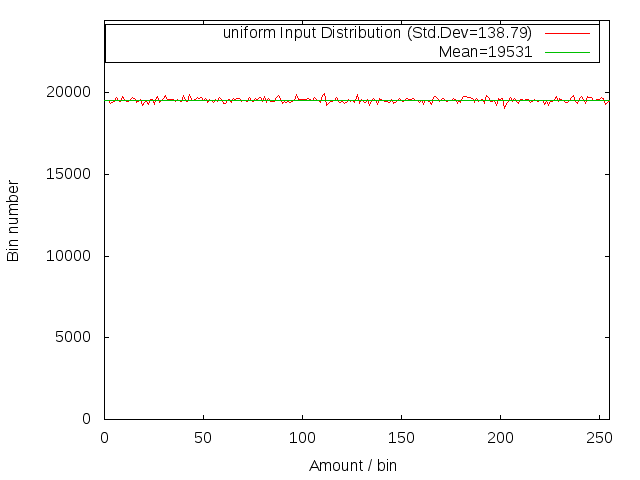
\includegraphics[width=\textwidth]{Graphs/Dist/Tabulation_uniform_dist.png}
    \caption{Uniform Input Distribution}
    \label{fig:tab_dist_uni}
  \end{subfigure}
\end{figure}
\begin{figure}[H]\ContinuedFloat
  \centering
  \begin{subfigure}[b]{\textwidth}
    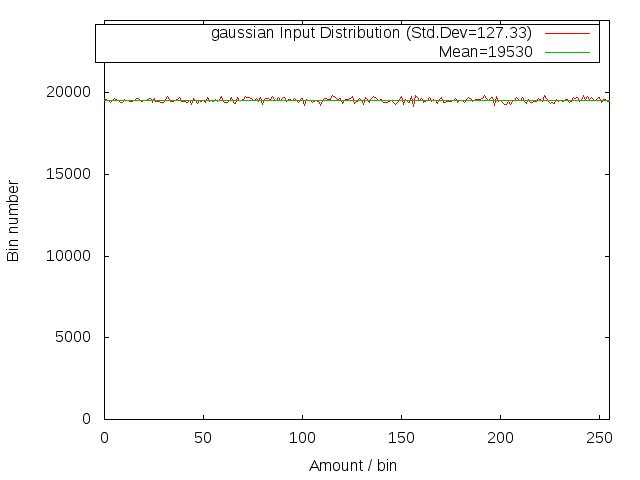
\includegraphics[width=\textwidth]{Graphs/Dist/Tabulation_gaussian_dist.png}
    \caption{Gaussian Input Distribution}
    \label{fig:tab_dist_gauss}
  \end{subfigure}
\end{figure}
\begin{figure}[H]\ContinuedFloat
  \centering
  \begin{subfigure}[b]{\textwidth}
    \includegraphics[width=\textwidth]{Graphs/Dist/Tabulation_zipfian_dist.png}
    \caption{Zipfian Input Distribution}
    \label{fig:tab_dist_exp}
  \end{subfigure}
  \caption{Output Distributions of Tabulation Hashing}\label{fig:tab_dist}
\end{figure}
\end{minipage}
\vfill
\columnbreak
\begin{minipage}{\columnwidth}
\begin{figure}[H]
    \centering
    \begin{subfigure}[b]{\textwidth}
        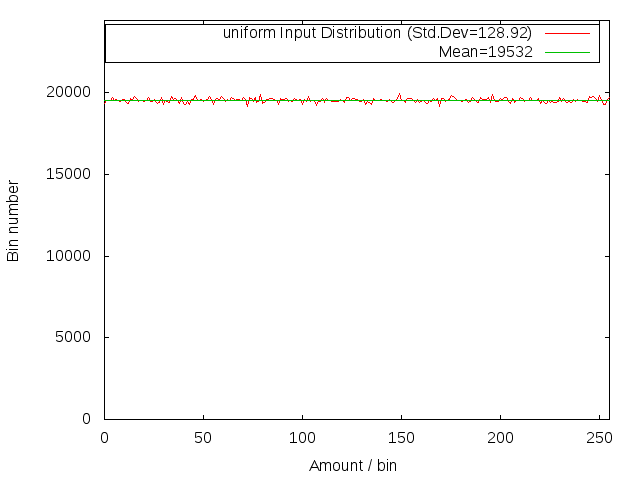
\includegraphics[width=\textwidth]{Graphs/Dist/Murmur_uniform_dist.png}
        \caption{Uniform Input Distribution}
        \label{fig:murmur_dist_uni}
    \end{subfigure}
\end{figure}
\begin{figure}[H]\ContinuedFloat
    \centering
    \begin{subfigure}[b]{\textwidth}
        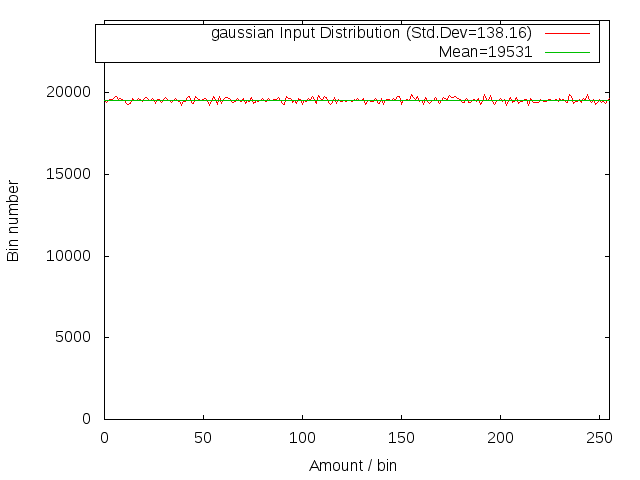
\includegraphics[width=\textwidth]{Graphs/Dist/Murmur_gaussian_dist.png}
        \caption{Gaussian Input Distribution}
        \label{fig:murmur_dist_gauss}
    \end{subfigure}
\end{figure}
\begin{figure}[H]\ContinuedFloat
    \centering
    \begin{subfigure}[b]{\textwidth}
        \includegraphics[width=\textwidth]{Graphs/Dist/Murmur_zipfian_dist.png}
        \caption{Zipfian Input Distribution}
        \label{fig:murmur_dist_exp}
    \end{subfigure}
    \caption{Output Distributions of Murmur Hashing}\label{fig:murmur_dist}
\end{figure}
\noindent
\end{minipage}
\end{multicols}
\noindent
At first glance, the output distribution of both hash functions for all three input distributions appears close to uniform, since the output distribution primarily lies within the upper and lower insignificant ranges. To validate this, we have performed a $\chi^2$ test, testing the likelihood that each of the output distributions was drawn from a uniform distribution around the mean. The following $p$ values have been found:

\begin{table}[htb]
\centering
\caption{p value for $\chi^2$ test on hashing distributions.}
\begin{tabular}{ | l || c | c | c |}
 \hline
 Input dist. & Uniform & Gaussian & Zipfian \\
 \hline
 Tabulation p value & 0.55 & 0.98 & 0.60  \\
 \hline
 Murmur p value & 0.94 & 0.59 & 0.83  \\
\hline
\end{tabular}
\label{tab:tab_dist}
\end{table}
\noindent
We can see that there is no statistical significant deviation from the assumed uniform distribution, since all of the found p values are greater than 0.05. Thus, both hash function are robust to skewed input distribution, producing close to uniform output distributions for all three used types of input distributions.
\\
Since both hash functions produce equally good output distributions, approximately the same amount of collision should occur. Thus, when using these in combination with a given hash index, the results should not be affected by one scenario having more collisions than the other. Therefore, if keeping all other factors besides the hash functions fixed, any difference in such results would be caused by one hash function having a higher throughput in the given scenario.

\subsection{Key-length experiment}
\label{subsec:hash_func_key_len}
To have a baseline of how well the two hash functions perform, a single threaded evaluation of the performance on various key lengths has been done, by hashing keys of different length and calculating the average runtime of each hash value computation. This experiment shows how well the implementation scales over key lengths, when used without any other structures. \\
\\
Since one of the key concepts of tabulation hashing is to utilize rapid lookups in fast cache, we have tried to use the L1 cache as little as possible for the generated keys, by only generating a small amount of strings (i.e., 5) for each of the lengths from 1-64 bytes, yielding 320 strings in total. For each of the 64 string lengths, the five strings have been hashed 10000 times, in order to make the total runtime long enough for the measurement to be stable. The duration of the repeated hash value computations have been measured using a high resolution clock that yields the total amount of nanoseconds used~\cite{chrono}. \\
\\
This entire setup has then been run 10000 times yielding a total of 100 million hash value computations of each string, from which average runtime and standard deviation can be calculated for each of the 64 lengths. \\
\\
Since tabulation hashing can be specialized for a given maximum key length, by tuning the amount of tables, this would be interesting to include in the experiment. Since more tabulation tables causes more contention of the cache, we expect using more tabulation tables to have a negative impact on the performance, while yielding more flexibility regarding the lengths of the keys used. To evaluate this hypothesis, we have run four separate runs for the tabulation hash function, using 8, 16, 32 and 64 tabulation tables, respectively. It should be noted that since tabulation hashing cannot hash keys longer than the amount of tabulation tables generated, each of the datasets only include data points up to the amount of tabulation tables employed. Only one run has been done for the murmur hash function, since it does not contain any tuning parameters. \\
\\
This experiment is interesting, as it shows an upper bound on how well the two hash functions can perform. The average runtime for each length can be seen in Figure \ref{fig:key_length}, which contains five curves, four for the four tabulation hashing runs using 8, 16, 32 and 64 tabulation tables, respectively, and one for the murmur hashing run. 

\begin{figure}[H]
  \centering
  \includegraphics[width=0.7\textwidth]{Graphs/Length/4_Tabulation_64_tables_length.png}\\
  \caption{Runtime of hash function invocations with different length input string.}\label{fig:key_length}
\end{figure}
\noindent
By first looking at the four data sets for the tabulation hash runs, we see that all of them experience a similar, close to linear degradation for short key lengths (i.e., up to 16 bytes). They all show the same runtime for hashing strings of just one byte, which takes roughly 6ns, while each additional byte in the string adds roughly 1.5ns.\\
\\
However, for the two runs using 32 and 64 tabulation tables respectively, we see that the scaling becomes less optimal for longer strings. Specifically, both of the two curves still show close to linear scaling for strings longer than 16 bytes, but with a steeper slope of roughly 2-2.5ns per additional byte. \\
\\
We believe that the steeper slope can be explained by looking at what the additional bytes cause to happen in the implementation. Since each byte causes a lookup in its own table, using longer strings will cause lookups in more tables. This in turn causes more cache lines to be loaded into the cache, which leads to more contention and therefore more cache misses. The overhead caused by this is however quite small.\\
\\
Secondly, it should be noted that while the four runs for tabulation hashing all appear close to linear, the standard deviation (seen on the error bars) increases as the amount of tables is increased, as well as when the length of the strings is increased. We believe this to be caused by the same contention of the cache as before.\\
\\
Finally, it can easily be seen that while the tabulation hashing has a slightly better performance on very short strings (i.e., up to three bytes), the murmur hash function scales better on the length of the key, since every four additional bytes in the key only increases the runtime of each hash function invocation by roughly 2ns: \\
\\
Murmur hashing takes \~10ns to hash a key of length one byte, and spends the same amount of time hashing strings of length up to four bytes. The increase in runtime thus only appears to happen after every fourth additional byte. This is caused by that the body loop of the murmur hashing implementation is iterated once for every 32-bit chunk of the key. It can thus be concluded that the increase in runtime primarily comes from additional iterations of this loop, while the difference between tails of length 0-3 bytes does not affect much.

\subsection{Multi-core experiment}
\label{subsec:hash_func_multi_core}
To evaluate the scalability across multiple cores, we have created an experimental setup similar to the key-length experiment (Figure~\ref{fig:key_length}), run it on multiple threads, and measured the throughput of each thread as well as the total throughput. This was done by initializing one hash function object,\footnote{Either of class \verb|tabulation_hash| or of class \verb|murmur_hash|} which is used by all the threads in their computations. Since the hash function objects are not modified after being initialized, this does not have any synchronization implications.y The threads are all pinned to a specific core to avoid reduced performance, e.g., from potentially having more cache misses. This pinning is done as explained in Section~\ref{subsec:hardware}. Each thread is given its own set of five strings, to avoid sharing of these memory regions. These strings are then hashed 100 million times, from which an average total throughput can be calculated. \\
\\
Since neither of the hash function classes contain any shared state which is modified after initialization, an optimal linear increase in throughput when utilizing more cores would be expected, if external factors are disregarded. However, as we have seen on Figure~\ref{fig:baseline_scaling}, external factors are in play. \\
\\
In Figure \ref{fig:tab_cores} the average total throughput is shown for both tabulation hashing and murmur hashing. As in the key-length experiment, we have included four curves for tabulation hashing, using 8, 16, 32 and 64 tabulation tables, respectively. Since the purpose of this experiment is to show how well the throughput of each of the configurations scale over multiple cores, the length of the keys has been fixed to be the maximum length possible, which is therefore equal to the number of tabulation tables for the tabulation hash sets, and 64 for the murmur hash set. \\
\\
Additionally, a linear function with slope equal to the throughput found when using just one thread has been added for each of the curves, which acts as reference for ideal scaling.\\

\begin{figure}[H]
  \centering
  \includegraphics[width=0.8\textwidth]{Graphs/Cores/4_Tabulation_8_tables_cores.png}\\
  \caption{Total throughput scalability of hash functions.}
  \label{fig:tab_cores}
\end{figure}
\noindent
While it might appear from this graph that tabulation hashing with eight tabulation tables has best overall performance, recall that this curve is generated by hashing keys of length 8, while all the other curves are generated by hashing longer keys. Similarly, while tabulation hashing with 16 tabulation tables and murmur hashing seem to have the same throughput, the former hashes keys of length 16, while the latter hashes keys of length 64. Therefore, since the goal of the graph is an understanding of the scalability of the setups, the curves should not be compared to each other.\\
\\
First note that all of the curves show three different linear sections (most apparent on the red curve), with different slopes. The first section shows very close to optimal scaling up to eight cores. In the next section (9-16 cores), the increase appears linear but with a reduced slope, thus indicating less optimal scaling. Finally, after 16 cores the scaling is reduced even further. \\
\\
To understand this behavior, recall the scalability behavior described in the hardware setup (Section~\ref{subsec:hardware}) on page~\pageref{subsec:hardware}. This scalability behavior very much resembles the behavior found with the dummy-workload, which indicates that the found scalability behavior of the hash functions is caused by the factors described there. \\
\\
Since we for different amounts of work of the dummy-workload have seen this exact behavior (i.e., 3 sections with only \~65\% of the ideal throughput found when using 32 cores), it would appear that the reduction in scalability is a percentage of the total throughput, instead of an absolute overhead. As such, a similar percentage wise reduction in performance is to be expected for these experiments. This is also emphasized by  comparing all five curves on Figure~\ref{fig:tab_cores} to their corresponding ideal scaling curve, which shows that they all exhibit 60-65\% of the ideal throughput for 32 cores.\\
\\
However, since we have no way of verifying that this is the sole cause of the reduced scaling, the primary take-away from the graph is the linear close to optimal scalability of all curves for the first eight cores. Whether or not the baseline scalability properties of the setup accounts for the entire reduction of throughput after eight cores cannot be determined.

\paragraph{Configuration of hash functions for the YCSB experiments.} Based on these hash function experiments, the following conclusion can be made: Both hash functions show good distributional properties, that should not have a negative impact on the performance of the hash indices. They are both able to handle variable length keys, but while both hash functions have comparably low runtime for short keys, the runtime for longer keys up to 64 bytes has been shown to be superior for murmur hashing. We expect this trend to extend beyond 64 bytes, as we have no indication of circumstances that changes this. \\
\\
It has, however, also been shown that using more tabulation tables does not increase the runtime of hashing short keys, compared to instantiating just enough tabulation tables. Such increase in runtime from using more tabulation tables is only seen when these tables are actually used, thus for longer keys. Additionally, we have seen similar scalability properties for all the tested configurations of hash functions. \\
\\
Overall, the two hash functions perform very similarly, with the primary difference being how fast they hash keys of different lengths. Since tabulation hashing is superior for short keys, it is preferable if a tight bound on the length of the keys is provided. However, as this is not generally the case, murmur hash appears as the optimal choice on most cases.\\
\\
The YCSB experiments on the hash indices have been performed with both hash functions, to evaluate the implication of the choice of hash function. In these experiments, tabulation hashing is configured to use 64 tables in the YCSB experiments, as this yields the highest degree of flexibility, without causing a trade-off in terms of performance. Since murmur hashing does not include any tuning parameters, it is used as it is.
\section{Experiments on hash indices}
\label{sec:hash_index_experiments}
In this section, we present the primary evaluation of the implemented hash indices. First, the experiments on how to tune the hash indices is presented and discussed in Section~\ref{subsec:tuning_experiments}. The results of these tuning experiments are used for the YCSB experiments on the hash indices. Secondly, the results of the running our YCSB implementation on the tuned hash indices is presented and discussed in Section~\ref{subsec:ycsb_results}.
\subsection{Tuning of hash indices for experiments}
\label{subsec:tuning_experiments}
We have chosen to only use the core workloads of the YCSB benchmark, and thus not use the provided extensibility to create new workloads, since we find that the core workloads properly exhaust the performance space, and that our hash indices did not have any specific characteristics that requires specialized experiments. Instead, we have identified the tuning parameters of the hash indices and performed experiments with these, to find an understanding of the trade-offs connected to these parameters.\\
\\
The tuning parameters are,
\begin{itemize}
  \item Maximum key length (tabulation tables), for tabulation hashing
  \item Directory size, for array hashing
  \item Initial global depth, for extendible hashing
  \item Prefix bits (number of partitions), for partitioned array hashing
\end{itemize}
In the following sections, each of these tuning parameters is evaluated one at a time. However, since the key-length experiment performed in Section~\ref{subsec:hash_func_key_len} already has evaluated the maximum key length, showing that using more tabulation tables does not reduce the performance of hashing shorter keys, this tuning parameter will not be evaluated again. 
\paragraph{Directory size (Array Hashing).} For the directory size of array hashing, inserting the same amount of entries into a larger directory means less entries in each bucket, as there will be more buckets to distribute the entries between. Since all the operations traverse the bucket for a given key, fewer entries in each bucket causes shorter runtimes for all of the operations, thus yielding an overall higher throughput. However, if there is no or very few entries in the buckets, increasing the directory size will not yield a performance improvement.\\
\\
The performance gain comes as a trade-off with memory usage. As each bucket has a memory overhead from the additional pointer to the bucket, as well as the additional vectors and locking primitive, more buckets cause more memory to be used. The memory overhead for each bucket is 87B, as we have seven pointers (28B) and two allocators (8B),\footnote{One pointer to the bucket, and two vectors (keys and values), each having three pointers and an allocator~\cite{vector}.} one spinlock (40B) and possibly one atomic flag (1B).\footnote{This is only included for the spinlock implementation.} Since both the key and the value of a single entry are strings, one entry could quickly amount up to as much memory. Thus, as long as the majority of the buckets are not empty once the database has been loaded up to an expected load, the memory overhead of the additional buckets is outweighed by the memory used by the actual data stored.\\
\\
To verify this, an experiment has been conducted, in which the directory size has been varied for values between $2^4$ and $2^{20}$. Since the change in performance is caused by the lower probing time, we have chosen to run this experiment over core workload \verb|C| (described in Section~\ref{background:ycsb_core_workload}), as this workload includes 100\% read-operations, which are expected to have the lowest runtimes. Using core workload \verb|C| thus yields tuning parameter results under the highest throughput of all the core workloads, i.e., under the heaviest contention of each bucket. This makes the results useful for the other workloads as well, as none of them will produce more contention on the buckets, which could potentially cause less optimal performance. Similarly, we have chosen to run the test on 32 threads, as this also increases the contention on the buckets. Choosing the highest bucket contention ensures that the tuned hash index will perform optimal, even in the worst case.\\
\\
As for all of the core workloads, the loading phase of core workload \verb|C| inserts 100000 data entries. This can be used to estimate an average amount of data entries in each bucket for the different directory sizes. The throughput as well as the peak memory usage for different directory sizes can be seen in Figure~\ref{fig:dir_size}.

\begin{figure}[H]
  \centering
  \includegraphics[width=0.7\textwidth]{Graphs/tabulation_hash_array_hash_table_workload_c_dir_size_spinlock.png}\\
  \caption{Total throughput and memory usage for directory sizes of array hashing.}\label{fig:dir_size}
\end{figure}
\noindent
By first interpreting the red curve for the throughput, we can see that relaxing the contention in the buckets certainly can yield a performance increase. However, as early as after a directory size of 8192 buckets (i.e. roughly 13 data entries in each bucket), we start to see a flattening of the throughput curve, indicating that the increase in throughput from increasing the directory size is diminishing. Also, after a directory size of 65536 (i.e, roughly 1.5 entries in each bucket on average), the performance does not change significantly, since further significant reduction in the traversal time through each bucket cannot occur.\\
\\
Secondly, we can see that the memory usage increases significantly, as the size of the directory grows larger than 16384 buckets. The total memory increase seen from a directory size of $2^4$ to a directory size of $2^{20}$ is 90MB, very similar to the calculated overhead, which adds up to $(2^{20}-2^{4})*87B$ = 91MB.\\
\\
Overall, we can conclude that the tuning of the directory size yields the expected trade-off between throughput and memory usage. For the YCSB experiments on array hashing, we are using a directory size of 65536 which has shown to yield close to optimal performance, while still employing low memory usage.
\paragraph{Initial global depth (extendible hashing).} The initial global depth of extendible hashing is quite similar to the directory size of array hashing, but with two key differences. \\
\\
First of all, the global depth defined is only valid initially, as the global depth can increase as part of insert operations. As such, poor choice of this tuning parameter can eventually be compensated for by the algorithm itself. Secondly, since the buckets have a fixed size in extendible hashing, there is a fixed upper limit on the traversal time. There is therefore never much contention in any buckets, which means that performance gain on the traversal times will be less significant.\\
\\
The primary advantage of choosing a proper value for the initial global depth comes from avoiding the slow path of the insert algorithm (as described in Section~\ref{subsec:design_extendible_hashing_locking} on page~\pageref{subsec:design_extendible_hashing_locking}), as a larger initial global depth makes splits of the directory less frequent. Since the slow path requires exclusive access to the entire directory (and thus the entire data structure), reducing the amount of runs through this portion of the code yields an increase in the insertion throughput. However, as we saw in Section~\ref{subsec:design_extendible_hashing_locking}, there is a low upper bound on the maximum amount of times the slow path can be taken. So, this performance increase will be quite insignificant over the course of many operations.\\
\\
A secondary performance increase in the insert operation comes from the fact that a bucket is instantiated for every entry in the preallocated directory. Thus, a higher initial global depth causes more buckets to be instantiated initially. These buckets will thus not have to be instantiated during the execution of actual work. The allocation of buckets is, however, not very expensive, causing also this performance increase to be insignificant. \\
\\
The bucket allocation scheme also means, however, that the initial memory overhead of an increased preallocation of the directory is just as large for extendible hashing as for array hashing. While a doubling of the directory as part of the slow path of an insertion operation only creates new pointers to the original buckets, the number of buckets initially generated is equal to the size of the directory, and thus directly linked to the initial global depth. \\
\\
Since the focus of the YCSB benchmark is evaluating the transaction phase, we have chosen to show what impact the initial global depth has on this phase. Since the performance increase is expected to be caused by the insert operation, we have designed a new workload that is completely similar to core workload C, except that it includes 100\% inserts. This makes the performance effect as visible as possible. However, since the loading phase causes a high number of inserts, most of the reduced throughput from a poor tuning of the initial global depth is expected to happen in this phase, and thus not included in the results.\\
\\
The resulting throughput and memory usage of running this experiment can be seen in Figure \ref{fig:global_depht}.

\begin{figure}[H]
  \centering
  \includegraphics[width=0.7\textwidth]{Graphs/murmur_hash_extendible_hash_table_workload_insert_global_depth_mutex_murmur.png}\\
  \caption{Total throughput and memory usage for various initial global depths of extendible hashing.}\label{fig:global_depht}
\end{figure}

Notice that even though the experiment has been designed to make the performance gain as visible as possible, we do not see any performance increase from the increased preallocation caused by a greater initial global depth. As mentioned, we believe this to be due to the fact that the compensation for the poor initial allocation takes place in the loading phase.\\
\\
Therefore, the choice of this tuning parameter does not show any significant effect. To make the comparison of the hash indices as adequate as possible, we have chosen an initial global depth of 16, which yields a directory size of 65536 buckets, thus equal to the directory size used for the tuning of array hashing. As seen in the memory curve, the initial memory usage for this configuration is almost as low as for any smaller initial global depth.

\paragraph{Prefix bits (partitioned array hashing).} For the partitioned array hashing, the primary tuning parameter is how many prefix bits of the key should be used for radix partitioning. This parameter directly dictates how many partitions are created, which in turn dictates the number of entries in each partition. A lower load on each partition yields a performance increase on all operations. For the \verb|get|, \verb|insert| and \verb|update| operations, fewer entries in the used partition yields a lower traversal time through the bucket. For the range scan operation, the possibility of elimination of some partitions (as described in Section~\ref{sec:design_partition_hash_index} on page~\pageref{sec:design_partition_hash_index}) reduces the number of entries to be searched. Since the reason for the partitioning of the hash index was improving the performance of the range scans, this experiment will be performed with core workload E. \\
\\
When the number of partitions is increased, the load in each partition decreases. The lower load can potentially lead to a situation in which smaller directories for each of the partitions would be optimal. This is especially the case for range scans, where having many large partitions causes more buckets to be evaluated. If the load in each partition is so low that many of the buckets are empty, the performance of the partitioned range scan could be lower than the performance of using just a single partition.\\
\\
Varying both the number of prefix bits and the directory size of the partitions would be a heterogeneous tuning test, which is out of the scope of this project, due to time constraints. We therefore only present results found using the same directory size for all partitions. To make the effect of the prefix bits most significant, we have chosen to make the directories of all partitions small (i.e., $2^8 = 256$ buckets in each directory), as this makes the initial contention greater. In this way, the cost of evaluating the entries  greatly outweighs the cost of accessing the buckets. However, for the runs using more prefix bits, in which more partitions are created, the load in each bucket will be decreased, causing the cost of accessing all the buckets to be a relevant factor. The results of the experiment can be seen in Figure~\ref{fig:prefix_bits}.

\begin{figure}[H]
  \centering
  \includegraphics[width=0.7\textwidth]{Graphs/tabulation_hash_partitioned_array_hash_table_workload_e_prefix_bits_new_dist_8.png}\\
  \caption{Total throughput and memory usage for increasing number of prefix bits of partitioned array hashing.}\label{fig:prefix_bits}
\end{figure}
\noindent
As seen in this figure, for the lower ranges of prefix bits, we indeed get a performance increase when increasing the number of prefix bits and thus employing more partitions. This performance increase is caused by higher granularity of the partitions, causing a larger fraction of the key space to be eliminated from the range scan. \\
\\
We see that the highest performance is achieved when using 12 prefix bits. In this configuration, we have $2^{12} = 4096$ partitions, each with 256 buckets yielding a total of $2^{12}*2^8 = 2^{20} \approx 1000000$ buckets. As mentioned in the methodology Section~\ref{subsec:methodology}, the number of entries loaded into the store for core workload E is 10000, meaning that on average, only one in every 100 of the buckets have a single entry, while every partition has 2.5 entries on average. This emphasizes how poorly an unordered store handles range scans, since it states that using a sorted array of hash indices, each with an extremely limited load, causes better performance than performing the full scans inside fewer partitions containing more entries. \\
\\
When using more than 12 prefix bits, we see that the performance starts to drop. In these configurations, we essentially have a sorted array of hash indices, each containing just one entry in total, which can be seen as an ordered index structure. Thus, when using more than 12 prefix bits, we cannot reduce the load on each partition more, and therefore does increasing the number of partitions only cause more buckets to be evaluated, causing a drop in the performance.\\
\\
The memory overhead of using more prefix bits can be seen not to be significant in the shown example, since the individual partitions are so small. When using 12 prefix bits, a peak memory usage of 172MB has been seen, which easily fits in main memory of all modern hardware. However, the memory usage is doubled for every additional prefix bit, making the increase in memory usage exponential. If using larger partitions, the memory footprint might become a relevant factor to consider. In the YCSB experiments on the partitioned array hashing, the prefix bits have been targeted at obtaining the maximum performance, and therefore set to 12.

\paragraph{Narrowing of configuration space}
The space of possible configurations is large. Since we use two hash functions, three hash indices, six core workloads, and two variations of locking schemes, the total configuration space is too large to be presented here. This section therefore presents a discussion of which subsets of this configuration space are of highest interest, before we proceed with a presentation and discussion of the experiments and their results.\\
\\
A general reduction of the configuration space can be made on the concurrency locking schemes. Throughout every test performed, we have found that using spinlocks instead of the shared mutexes (as described in Section~\ref{subsec:design_locking_primitives} on page~\pageref{subsec:design_locking_primitives}) does not affect the single core performance of any of the operations in any of the hash indices, but impacts the scalability of the different hash indices. Specifically, using a spinlock for the local bucket locks yield improved scalability of throughput on all operations of all hash indices, while using a spinlock for the directory lock of extendible hashing yields reduced scalability of throughput on all operations. \\
\\
This complies with the theoretical discussion of which locking primitive to use for the global and local locks presented in Section~\ref{subsec:design_locking_primitives}. The results presented in Section~\ref{subsec:ycsb_results} have thus been generated using the spinlock implementation for the local bucket locks and a \verb|shared_mutex| for the directory lock.\\
\\
While using a \verb|shared_mutex| for the directory lock is advantageous over using the spinlock implementation, the high contention on the \verb|shared_mutex| makes the costs of giving the control to the operating system very high. This has been verified in the following experiment, where the throughput of running core workload F on extendible hashing, using the spinlock and shared mutex implementations respectively, is compared. Core workload F only contains reads and updates, and does thus never cause exclusive access mode to the directory lock to be taken. The of this experiment can be seen in Figure~\ref{fig:extendible_lock_comparison}.

\begin{figure}[H]
  \centering
  \includegraphics[width=0.7\textwidth]{Graphs/extendible_lock_comparison_f.png}\\
  \caption{Total throughput for the two locking primitives on the directory lock, using workload F.}\label{fig:extendible_lock_comparison}
\end{figure}
\noindent
The scalability of both locking primitives can be seen to be very poor. The contention on the spinlock can be seen to have the greatest impact on the performance, as the performance quickly drops below the single threaded performance. For the \verb|shared_mutex| implementation, the performance impact caused by contention also eliminates scaling of throughput on multiple cores, as the performance when using more than five cores is comparable with the single threaded performance.\\
\\
For range scans, the critical section is longer, meaning that each operation takes longer to complete. The contention on the directory lock is therefore lower when the fraction of range scan operations is higher. Running the same experiment on core workload E, in which 95\% of the operations are range scans, the advantage of using a \verb|shared_mutex| for the directory lock is expected to be amplified. The results of this experiment can be seend in Figure~\ref{fig:extendible_lock_comparison_e}.

\begin{figure}[H]
  \centering
  \includegraphics[width=0.7\textwidth]{Graphs/extendible_lock_comparison_e.png}\\
  \caption{Total throughput for the two locking primitives on the directory lock, using workload E.}\label{fig:extendible_lock_comparison_e}
\end{figure}
\noindent
In this figure, we observe some degree of scalability for extendible hashing when a \verb|shared_mutex| is used for the directory lock. The longer critical sections of the operations of this experiment causes less contention on the directory lock, since the throughput of operations will be lower. Since the longer critical sections is the main difference between the experiments of Figure~\ref{fig:extendible_lock_comparison} and Figure~\ref{fig:extendible_lock_comparison_e}, we believe that the high contention of the directory lock is the main cause of the poor scalability of extendible hashing.\\
\\
Overall, these results show that pessimistic concurrency control overall is very unfitting for the global mutable directory of extendible hashing. However, since the best results have been found using the \verb|shared_mutex| implementation, all results shown have been created using this locking primitive for the directory lock. This narrows down the configuration space, leaving 36 combinations of the two hash functions, three hash indices and six core workloads. \\
\\
To easily compare the performance of the hash indices, we plot these three on the same graph, thus yielding a total of 12 graphs. Additionally, to easily compare the impact of the choice of hash function, we present pair of graphs for the hash functions side by side.\footnote{Note: If some details are difficult to read from the small graphs, we refer to Appendix~\ref{appendix:full_result_overview} for full size graphs.} Finally, since each of the six core workloads are designed to simulate a characteristic workload for certain applications, we have found showing the results of all six core workloads relevant. 
\subsection{YCSB core workload results}
\label{subsec:ycsb_results}
The experiments with the core workloads of YCSB is presented in an order that makes showing certain features of the implementation easiest, and thus not in the alphabetic order. 

In common for all six pairs of graphs, we shall soon see that the two graphs of each pair are very similar. This suggests that the runtime of the hash functions is insignificant in the overall picture. The discussion on each pair of graphs therefore primarily regards the three hash indices. Additionally, since high contention on the directory lock of extendible hashing hinders any scaling, this hash index is only discussed when other interesting features show.

\paragraph{Core workload C.} Core workload C is a read only workload, thus consisting of 100\% reads. This workload thus yields an understanding of how well the implemented hash indices throughput scale over multiple cores, since not a single data entry is modified after the loading phase. \\
\\
The results can be seen in Figure~\ref{fig:res_c}. The maximum throughput for each configuration is shown on the legend (in parentheses).

\begin{figure}[ht]
  \centering
  \begin{subfigure}[b]{0.45\textwidth}
    \includegraphics[width=\textwidth]{Graphs/murmur_hash_workload_c_spinlock_16_8_12_large.png}
    \caption[]{Murmur hashing.}
    \label{fig:mur_c}
  \end{subfigure} \hfill
  \begin{subfigure}[b]{0.45\textwidth}
    \includegraphics[width=\textwidth]{Graphs/tabulation_hash_workload_c_spinlock_16_8_12_large.png}
    \caption[]{Tabulation hashing.}
    \label{fig:tab_c}
  \end{subfigure}
  \caption[]{Throughput results for core workload C.}
  \label{fig:res_c}
\end{figure}
\noindent
Array hashing and partitioned array hashing can be seen to show very similar results, for both murmur hashing and tabulation hashing. For all four configurations, a close to ideal scaling can be seen for the first eight cores, yielding a throughput of roughly 5.75 million operations per second using eight cores. Additionally, using up to 13 cores also show good scaling properties for both hash indices. The maximum throughput is in all four configurations found at 13 cores, and is quite similar for all four configurations,  in the range of 7.07-7.37 million operations per second. The peak performance of the two hash functions is very similar, with murmur hashing showing a minor advantage over tabulation hashing. This in accordance with the hash function experiments presented in Section~\ref{sec:hash_func_experiments}. \\
\\
Additionally, we can see a minor peak performance advantage of partitioned array hashing over array hashing, as the peak throughput when using partitioned array hashing is roughly 3\% higher than when using array hashing, for both hash functions. Additionally, by evaluating the curves for array hashing and partitioned array hashing, this minor performance advantage seems to be present for the majority of the data points up to 13 cores.\\
\\
However, when using more than 13 cores, we see that the performance of all four configurations quickly drops to a level comparable to using four cores (at 16 cores), and from there slowly decreases towards the performance of just two cores. We believe this drop in performance to be caused by contention on the bucket locks. \\
\\
This hypothesis can be emphasized by evaluating the experiments of the other core workload. Specifically, since the read operations are expected to be fastest, as it does not cause any memory writes, including other operations is expected to cause a lower total throughput. The lower throughput will cause less contention, which we expect to cause the drop in performance to happen after more cores have been employed.
\paragraph{Core workload B and D.} 
Since both core workload B and D contain 95\% reads, with 5\% updates and writes respectively, the experiments using these core workloads will be presented together in this paragraph. Besides the operation selection of the remaining 5\%, the only difference between them is the key generation distribution, which for core workload B is zipfian, while core workload D uses their \verb|latest| distribution.\\
\\
The results found for the two workloads are also quite similar, and will be presented in succession in Figure~\ref{fig:res_b} and Figure~\ref{fig:res_d} and discussed together.\\
\begin{figure}[H]
  \centering
  \begin{subfigure}[b]{0.45\textwidth}
    \includegraphics[width=\textwidth]{Graphs/murmur_hash_workload_b_spinlock_16_8_12_large.png}
    \caption[]{Murmur hashing.}
    \label{fig:mur_b}
  \end{subfigure} \hfill
  \begin{subfigure}[b]{0.45\textwidth}
    \includegraphics[width=\textwidth]{Graphs/tabulation_hash_workload_b_spinlock_16_8_12_large.png}
    \caption[]{Tabulation hashing.}
    \label{fig:tab_b}
  \end{subfigure}
  \caption[]{Throughput results for core workload B.}
  \label{fig:res_b}
\end{figure}
\begin{figure}[H]
  \centering
  \begin{subfigure}[b]{0.45\textwidth}
    \includegraphics[width=\textwidth]{Graphs/murmur_hash_workload_d_spinlock_16_8_12_large.png}
    \caption[]{Murmur hashing.}
    \label{fig:mur_d}
  \end{subfigure} \hfill
  \begin{subfigure}[b]{0.45\textwidth}
    \includegraphics[width=\textwidth]{Graphs/tabulation_hash_workload_d_spinlock_16_8_12_large.png}
    \caption[]{Tabulation hashing.}
    \label{fig:tab_d}
  \end{subfigure}
  \caption[]{Throughput results for core workload D.}
  \label{fig:res_d}
\end{figure}
\noindent
In all four figures, we see close to ideal throughput scaling for the first eight cores. However, for both hash indices on all four of these graphs, the single core performance is lower than for workload C, which means when using eight cores, we see a throughput of roughly 5 million operations per second, thus roughly
13\% lower throughput than what was found for workload C, using the same amount of cores.\\
\\
The slightly lower throughput can also be seen by looking at the maximum throughputs which for all eight configurations is between 6.44-6.69 million operations per second, thus 9-10\% lower than the maximum throughput of the experiment with core workload C. However, for core workload B we see no pattern between which hash function or hash index achieves the highest performance, while tabulation hashing yields a slightly higher maximum performance than murmur hashing for core workload D. \\
\\
Also similar to the experiment using workload C, we see an increase in throughput when using more than eight cores. However, for seven of the eight configurations presented on these graphs (excluding partitioned array hashing using murmur hashing for workload B), we see that the maximum throughput is achieved using 14 cores, thus when employing one more core than for the maximum throughput of workload C. \\
\\
Since the throughput of these experiments is slightly lower than the throughput for the core workload C experiments, the fact that the drop happens when employing an additional core is in accordance with the proposed hypothesis of why the drop happens. Specifically, with the lower throughput, the contention on the bucket locks will be lower, thus requiring more cores to be employed, before contention causes the performance to drop.\\
\\
The hypothesis can be further emphasized by evaluating core experiment A and F, which both only employ 50\% reads, with the remaining 50\% of the operations being updates and read-modify-update operations, respectively. For these experiments, we expect lower throughput, which in turn is expected to enable more cores to be employed, before the performance drops.
\paragraph{Core workload A.} Core workload A is an update heavy workload, in which half of the operations are updates, while the other half is reads. A session store that records recent actions is an example of an application for which such workload is common. 
\begin{figure}[ht]
  \centering
  \begin{subfigure}[b]{0.45\textwidth}
    \includegraphics[width=\textwidth]{Graphs/murmur_hash_workload_a_spinlock_16_8_12_large.png}
    \caption[]{Murmur hashing.}
    \label{fig:mur_a}
  \end{subfigure} \hfill
  \begin{subfigure}[b]{0.45\textwidth}
    \includegraphics[width=\textwidth]{Graphs/tabulation_hash_workload_a_spinlock_16_8_12_large.png}
    \caption[]{Tabulation hashing.}
    \label{fig:tab_a}
  \end{subfigure}
  \caption[]{Throughput results for core workload A.}
  \label{fig:res_a}
\end{figure}

\paragraph{Core workload F.} 
\begin{figure}[ht]
  \centering
  \begin{subfigure}[b]{0.45\textwidth}
    \includegraphics[width=\textwidth]{Graphs/murmur_hash_workload_f_spinlock_16_8_12_large.png}
    \caption[]{Murmur hashing.}
    \label{fig:mur_f}
  \end{subfigure} \hfill
  \begin{subfigure}[b]{0.45\textwidth}
    \includegraphics[width=\textwidth]{Graphs/tabulation_hash_workload_f_spinlock_16_8_12_large.png}
    \caption[]{Tabulation hashing.}
    \label{fig:tab_f}
  \end{subfigure}
  \caption[]{Throughput results for core workload F.}
  \label{fig:res_f}
\end{figure}

\paragraph{Core workload E.} 
\begin{figure}[ht]
  \centering
  \begin{subfigure}[b]{0.45\textwidth}
    \includegraphics[width=\textwidth]{Graphs/murmur_hash_workload_e_spinlock_16_8_12_large.png}
    \caption[]{Murmur hashing.}
    \label{fig:mur_e}
  \end{subfigure} \hfill
  \begin{subfigure}[b]{0.45\textwidth}
    \includegraphics[width=\textwidth]{Graphs/tabulation_hash_workload_e_spinlock_16_8_12_large.png}
    \caption[]{Tabulation hashing.}
    \label{fig:tab_e}
  \end{subfigure}
  \caption[]{Throughput results for core workload E.}
  \label{fig:res_e}
\end{figure}




\chapter{Discussion}
\label{chap:discussion}
Subjective evaluation of results\\
Further work
\begin{itemize}
  \item Finer granularity of locks (entry locks)
  \item Optimistic concurrency control
\end{itemize}
\chapter{Conclusion}
\label{chap:conclusion}

\appendix
\chapter{Results in full size}
\label{appendix:full_result_overview}
\begin{figure}[H]
  \centering
  \includegraphics[width=\textwidth]{Graphs/tabulation_hash_workload_a_spinlock_16_8_12.png}\\
  \caption[]{Throughput for workload A, using tabulation hashing.}\label{fig:tab_a_full}
\end{figure}
\begin{figure}[H]
  \centering
  \includegraphics[width=\textwidth]{Graphs/tabulation_hash_workload_b_spinlock_16_8_12.png}\\
  \caption[]{Throughput for workload B, using tabulation hashing.}\label{fig:tab_b_full}
\end{figure}
\begin{figure}[H]
  \centering
  \includegraphics[width=\textwidth]{Graphs/tabulation_hash_workload_c_spinlock_16_8_12.png}\\
  \caption[]{Throughput for workload C, using tabulation hashing.}\label{fig:tab_c_full}
\end{figure}
\begin{figure}[H]
  \centering
  \includegraphics[width=\textwidth]{Graphs/tabulation_hash_workload_d_spinlock_16_8_12.png}\\
  \caption[]{Throughput for workload D, using tabulation hashing.}\label{fig:tab_d_full}
\end{figure}
\begin{figure}[H]
  \centering
  \includegraphics[width=\textwidth]{Graphs/tabulation_hash_workload_e_spinlock_16_8_12.png}\\
  \caption[]{Throughput for workload E, using tabulation hashing.}\label{fig:tab_e_full}
\end{figure}
\begin{figure}[H]
  \centering
  \includegraphics[width=\textwidth]{Graphs/tabulation_hash_workload_f_spinlock_16_8_12.png}\\
  \caption[]{Throughput for workload F, using tabulation hashing.}\label{fig:tab_f_full}
\end{figure}
\begin{figure}[H]
  \centering
  \includegraphics[width=\textwidth]{Graphs/murmur_hash_workload_a_spinlock_16_8_12.png}\\
  \caption[]{Throughput for workload A, using murmur hashing.}\label{fig:mur_a_full}
\end{figure}
\begin{figure}[H]
  \centering
  \includegraphics[width=\textwidth]{Graphs/murmur_hash_workload_b_spinlock_16_8_12.png}\\
  \caption[]{Throughput for workload B, using murmur hashing.}\label{fig:mur_b_full}
\end{figure}
\begin{figure}[H]
  \centering
  \includegraphics[width=\textwidth]{Graphs/murmur_hash_workload_c_spinlock_16_8_12.png}\\
  \caption[]{Throughput for workload C, using murmur hashing.}\label{fig:mur_c_full}
\end{figure}
\begin{figure}[H]
  \centering
  \includegraphics[width=\textwidth]{Graphs/murmur_hash_workload_d_spinlock_16_8_12.png}\\
  \caption[]{Throughput for workload D, using murmur hashing.}\label{fig:mur_d_full}
\end{figure}
\begin{figure}[H]
  \centering
  \includegraphics[width=\textwidth]{Graphs/murmur_hash_workload_e_spinlock_16_8_12.png}\\
  \caption[]{Throughput for workload E, using murmur hashing.}\label{fig:mur_e_full}
\end{figure}
\begin{figure}[H]
  \centering
  \includegraphics[width=\textwidth]{Graphs/murmur_hash_workload_f_spinlock_16_8_12.png}\\
  \caption[]{Throughput for workload F, using murmur hashing.}\label{fig:mur_f_full}
\end{figure}


\begin{thebibliography}{99}

\bibitem{MT12}
 Mao, Y.; Kohler, E.; Robert, M. (2012) \\
 \emph{Cache Craftiness for Fast Multicore Key-Value Storage}\\
 http://doi.acm.org/10.1145/2168836.2168855

\bibitem{SILO13}
 Tu, S.; Zheng, W.; Kohler, E.; Liskov, B.; Madden, S. (2013) \\
 \emph{Speedy Transactions in Multicore In-Memory Databases} \\
 http://doi.acm.org/10.1145/2517349.2522713

\bibitem{Zobrist}
 Zobrist, A. (1970)\\
 \emph{A New Hasahing Method with Application for Game Playing.}\\
 http://research.cs.wisc.edu/techreports/1970/TR88.pdf

\bibitem{WC79}
 Carter, J.; Wegman, Mark. (1979)\\
 \emph{Universal classes of hash functions.}\\
 Journal of Computer and System Sciences, 143-154:\\
 https://www.cs.princeton.edu/courses/archive/fall09/cos521/Handouts/universalclasses.pdf

\bibitem{WC81}
 Carter, J.; Wegman, Mark. (1981)\\
 \emph{New Hash Functions and Their Use in Authentication and Set Equality}
 http://www.fi.muni.cz/~xbouda1/teaching/2009/IV111/Wegman\_Carter\_1981\_New\_hash\_functions.pdf

\bibitem{TZ09}
 Thorup, M.; Zhang, Y. (2009)\\
 \emph{Tabulation based 5-universal hashing and linear probing.}\\
 In Proc. 12th Workshop on Algorithm Engineering and Experiments (ALENEX), 2009

\bibitem{PT11}
 Pătraşcu, M.; Thorup, M. (2011)\\
 \emph{The Power of Simple Tabulation Hashing}\\
 http://arxiv.org/abs/1011.5200

\bibitem{RAD15} % 0
 Richter, S.; Alvarez, V.; Dittrich, J. (2015)\\
 \emph{A seven Dimensional Analysis of Hashing Methods and its Implications on Query Processing}\\
 http://www.vldb.org/pvldb/vol9/p96-richter.pdf

% Hash Tables
\bibitem{ItA09}
 Cormen, Thomas H.; Leiserson, Charles E.; Rivest, Ronald L.; Stein, Clifford (2009). \\
 \emph{Introduction to Algorithms (3rd ed.).} \\
 Massachusetts Institute of Technology. pp. 253–280. ISBN 978-0-262-03384-8.

\bibitem{ItA092}
 Cormen, Thomas H.; Leiserson, Charles E.; Rivest, Ronald L.; Stein, Clifford (2009). \\
 \emph{Introduction to Algorithms (3rd ed.).} \\
 Massachusetts Institute of Technology. pp. 257–260. ISBN 978-0-262-03384-8.

\bibitem{NA09} % 1
 Askitis, N. (2009)\\
 \emph{Fast and Compact Hash Tables for Integer Keys}\\
 http://dl.acm.org/citation.cfm?id=1862675

\bibitem{AJ05}
 Askitis, N.; Zobel, J. (2005)\\
 \emph{Cache-Conscious Resolution in String Hash Tables}
 http://goanna.cs.rmit.edu.au/~jz/fulltext/spire05.pdf

\bibitem{ADSJ13} % 6
 Dudás, Á.; Juhasz, S. (2013)\\
 \emph{Blocking and non-blocking concurrent hash tables in multi-core systems}\\
 http://www.wseas.org/multimedia/journals/computers/2013/5705-125.pdf

\bibitem{BC10}
 Cooper, B. F.; Silberstein, A.; Tam, E.; Ramakrishnan, R.; Sears, R. (2010)\\
 \emph{Benchmarking Cloud Serving Systems with YCSB}\\
 https://www.cs.duke.edu/courses/fall13/cps296.4/838-CloudPapers/ycsb.pdf

\bibitem{BCycsb}
 Cooper, B.\\
 \emph{Yahoo! Cloud Serving Benchmark}\\
 https://github.com/brianfrankcooper/YCSB

\bibitem{FNV}
 \emph{Fowler-Noll-Vo hash function}\\
 https://en.wikipedia.org/wiki/Fowler\%E2\%80\%93Noll\%E2\%80\%93Vo\_hash\_function
  
\bibitem{Mur3}
 Appleby, A.\\
 \emph{Original Murmurhash3 implementation}\\
 https://github.com/aappleby/smhasher, version 08/01/16

\bibitem{DPH90}
 Dietzfelbinger, Martin, et al. (1994)\\
 \emph{Dynamic perfect hashing: Upper and lower bounds.}\\
 SIAM Journal on Computing 23.4 (1994): 738-761.

\bibitem{nphf}
 \emph{Napoleon machine, for the HIPERFIT research center}\\
 http://napoleon.hiperfit.dk/

\bibitem{dms03}
 Ramakrishnan, Raghu.; Gehrke, J. (2003)\\
 \emph{Database Management Systems, Extendible Hashing}\\
 Database Management Systems, 3rd edition: 738-761.

\bibitem{radix}
 Polychroniou, O.; Ross, K. (2014)\\
 \emph{A Comprehensive Study of Main-Memory Partitioning and its Application to Large-Scale Comparison- and Radix-Sort}\\
 http://www.cs.columbia.edu/~orestis/sigmod14I.pdf

\bibitem{ARTful}
 Leis, V.; Kemper, A.; Neumann, T. (2013)\\
 \emph{The Adaptive Radix Tree: ARTful Indexing for Main-Memory Databases}\\
 http://dx.doi.org/10.1109/ICDE.2013.6544812

\bibitem{silt11}
 Lim, H.; Fan, B.; Andersen, D.; Kaminsky, M. (2011)\\
 \emph{SILT: A Memory-Efficient, High-Performance Key-Value Store}\\
 https://www.cs.cmu.edu/~dga/papers/silt-sosp2011.pdf

\bibitem{db_ranking}
 \emph{DB-engines Ranking of Key Value Stores}\\
 http://db-engines.com/en/ranking/key-value+store

\bibitem{cassandra}
 \emph{Apache Cassandra Database}\\
 http://cassandra.apache.org/

\bibitem{redis}
 \emph{Redis data structure store}\\
 http://redis.io/

\bibitem{oracle}
 \emph{Oracle NoSQL Database}\\
 http://www.oracle.com/technetwork/database/database-technologies/nosqldb/overview/index.html

\bibitem{hbase}
 \emph{Apache HBase Hadoop Database} \\
 https://hbase.apache.org/

\bibitem{dynamo}
 DeCandia, G. et al. (2007)\\
 \emph{Dynamo: Amazon’s Highly Available Key-value Store}\\
 http://www.allthingsdistributed.com/files/amazon-dynamo-sosp2007.pdf

\bibitem{memcached}
 \emph{Memcached in-memory key-value store}\\
 http://www.memcached.org/

\bibitem{HFTP}
 \emph{Hadoop filesystem implementation}\\
 https://hadoop.apache.org/docs/r1.2.1/hftp.html

\bibitem{MT02}
 Matsumoto, M.; Nishimura, T. (2002) \\
 \emph{Mersenne Twister Home Page} \\
 http://www.math.sci.hiroshima-u.ac.jp/~m-mat/MT/emt.html

\bibitem{chrono}
 \emph{Chrono high resolution clock} \\
 http://en.cppreference.com/w/cpp/chrono/high\_resolution\_clock

\bibitem{vector}
 \emph{Vector implementation used}\\
 http://en.cppreference.com/w/cpp/container/vector

\bibitem{boost_shared_mutex}
 \emph{Boost Shared Mutex documentation}\\
 http://www.boost.org/doc/libs/1\_58\_0/doc/html/thread/synchronization.html\#thread.synchronization.mutex\_types.shared\_mutex

\bibitem{boost_mutex}
 \emph{Boost Mutex documentation}\\
 http://www.boost.org/doc/libs/1\_58\_0/doc/html/thread/synchronization.html\#thread.synchronization.mutex\_types.mutex

\bibitem{atomic_flag}
 \emph{Standard Library Atomic Flag documentation}\\
 http://en.cppreference.com/w/cpp/atomic/atomic\_flag

\bibitem{spinlock}
 Boddaert, G. \\
 \emph{User-Level Spin Locks} \\
 http://www.codeproject.com/Articles/784/User-Level-Spin-Locks
\end{thebibliography}
\end{document}
